\chapter{Alloy Manufacture}

It is well understood that the manufacturing route used to produce engineering components, especially for aerospace, is able to produce components with optimised properties and for this reason thermomechanical processing, despite its high cost, is preferred over casting in critical components.  In this chapter, we demonstrate that a robust route to manufacture is essential even at this early stage of development.  In this work, the lack of a robust route due to cost constraints has unfortunately been proven critical to the evaluation of these materials.  This chapter has been organised into: outlining the reasons for our choice in manufacturing routes, describing the non-directional and directional manufacturing routes explored, and summarising our findings in manufacture.

\section{Exploration of Alloy Manufacturing Routes}

Silicides are conventionally manufactured by hot isostatically pressing powder to achieve superior mechanical properties to arc-melted ingots.  This allows for a very fine, isotropic microstructure, and has been shown to result in effective load-partitioning into the intermetallic phase with the appropriate manufacturing conditions. 

Hot isostatic press is an expensive batch process, especially in the initial stages of experimental alloy design, where many alloys need to be explored empirically rather than designing many virtual alloys and manufacturing only one alloy.  It would have been ideal to process a representative base alloy of the explored system by both routes to determine the route that would produce a superior product.  Unfortunately, hot isostatic press manufacture was not pursued for several reasons.  A single batch of alloy powder would have cost thousands of pounds to make.  This would be a small batch of bespoke novel alloy, and there is a substantial probability that product quality could be questionable, seeing as the powder-producers would have no experience in milling this powder.  Grain size distribution would probably be wide.  The conditions required for hot isostatic press manufacture would need to be determined, as we have no experiences in pressing such powders.  The influence on powder quality and hot press conditions would be significant.  It was thought that the return on investment would not be high.  Hot isostatic press manufacture was thus not pursued as the main route of alloy manufacture.

DS manufactured eutectic alloy would have a lamellar microstructure which may improve fracture-toughness by increasing critical crack length through crack deflection.  Having the load-bearing intermetallic phase aligned along the loading-axis may be a good microstructure for withstanding load.

We thought it sensible to compare the mechanical properties of a base alloy manufactured through both directional solidified and hot isostatic press manufacture in the first instance to determine the superior route.  Due to limited funds and access to equipment, alloys could only be DS manufactured.  We will describe how this route of manufacture had limited success due to furnace limitations.


\section{Non-Directional Alloy Manufacture}

\subsection{Arc-Melt Manufacture} 

Arc-melt ingots were used in the initial exploration of potential compositions.  This method allows small, relatively isotropic ingots to be made up with ease, provided that the components are miscible, do not have vastly different melting points, and do not form intermediate phases that have very high melting points of above 2500\celsius.  

The in-house arc-melt machine available in-house is 20 years old and manufactured by Buehler.  It is operated by Mr Kevin Roberts, a technician that has decades of experience with arc-melting.  Ingots weighed between 15-45 \gram, and were slug-like, measuring 7-12 \centi\metre\ in length (Figure \ref{fig:crarc}).  After the first pass of the arc, ingots were flipped and re-melted twice more.

Most alloy melts flowed poorly under the arc.  Compositions containing chromium and silicon would crack into several pieces during the fast cooling rates typical of arc-melt manufacture (Figure \ref{fig:crarc}).  Adjacent grains in the ingots were found to possess vastly different microstructures, with one having a lamellar microstructure, and its neighbour comprising mostly of dendrites.  In some regions, unmelted bits of elemental stock were seen.  Silicon and silicides make for very viscous material that has poor mixability.  In other regions where unmelted stock is not seen, the non-lamellar microstructures may be a result of different undercooling rates experienced by a melt of eutectic composition.  For instance, if the degree of undercooling is too big, the melt will solidify into a melt containing pro-eutectic, as seen in Figure \ref{fig:dantzig}.

%
\begin{figure}[H]
\begin{center}
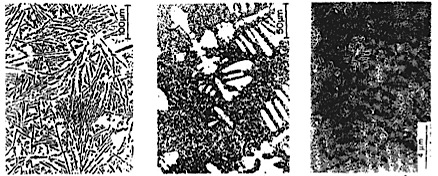
\includegraphics[width=10cm]{coolingrate}
\caption{Effect of undercooling on the microstructure of Al--Si alloys: (a) Eutectic composition, slow cooling, (b) euctectic composition, fast cooling, (c) hypereutectic composition, laser re-melted at 0.1\metre/s.}
\label{fig:dantzig}
\end{center}
\end{figure}
%
Regardless of whether the ingots are compositionally homogeneous, the ingots manufactured by the arc-melt process are intrinsically microstructurally inhomogeneous.  This cannot be homogenised or optimised in any reasonable fashion, and these ingots cannot be used for high-temperature mechanical testing of any sensible nature.  Besides, rampant sample cracking upon cooling from manufacture indicate that arc-melt material experience residual cooling stresses that are of substantial magnitude to cause catastrophic failure.  Even if an ingot did not crack during cooling, it would be prone to cracking during handling and machining.

%
\begin{figure}[H]
\begin{center}
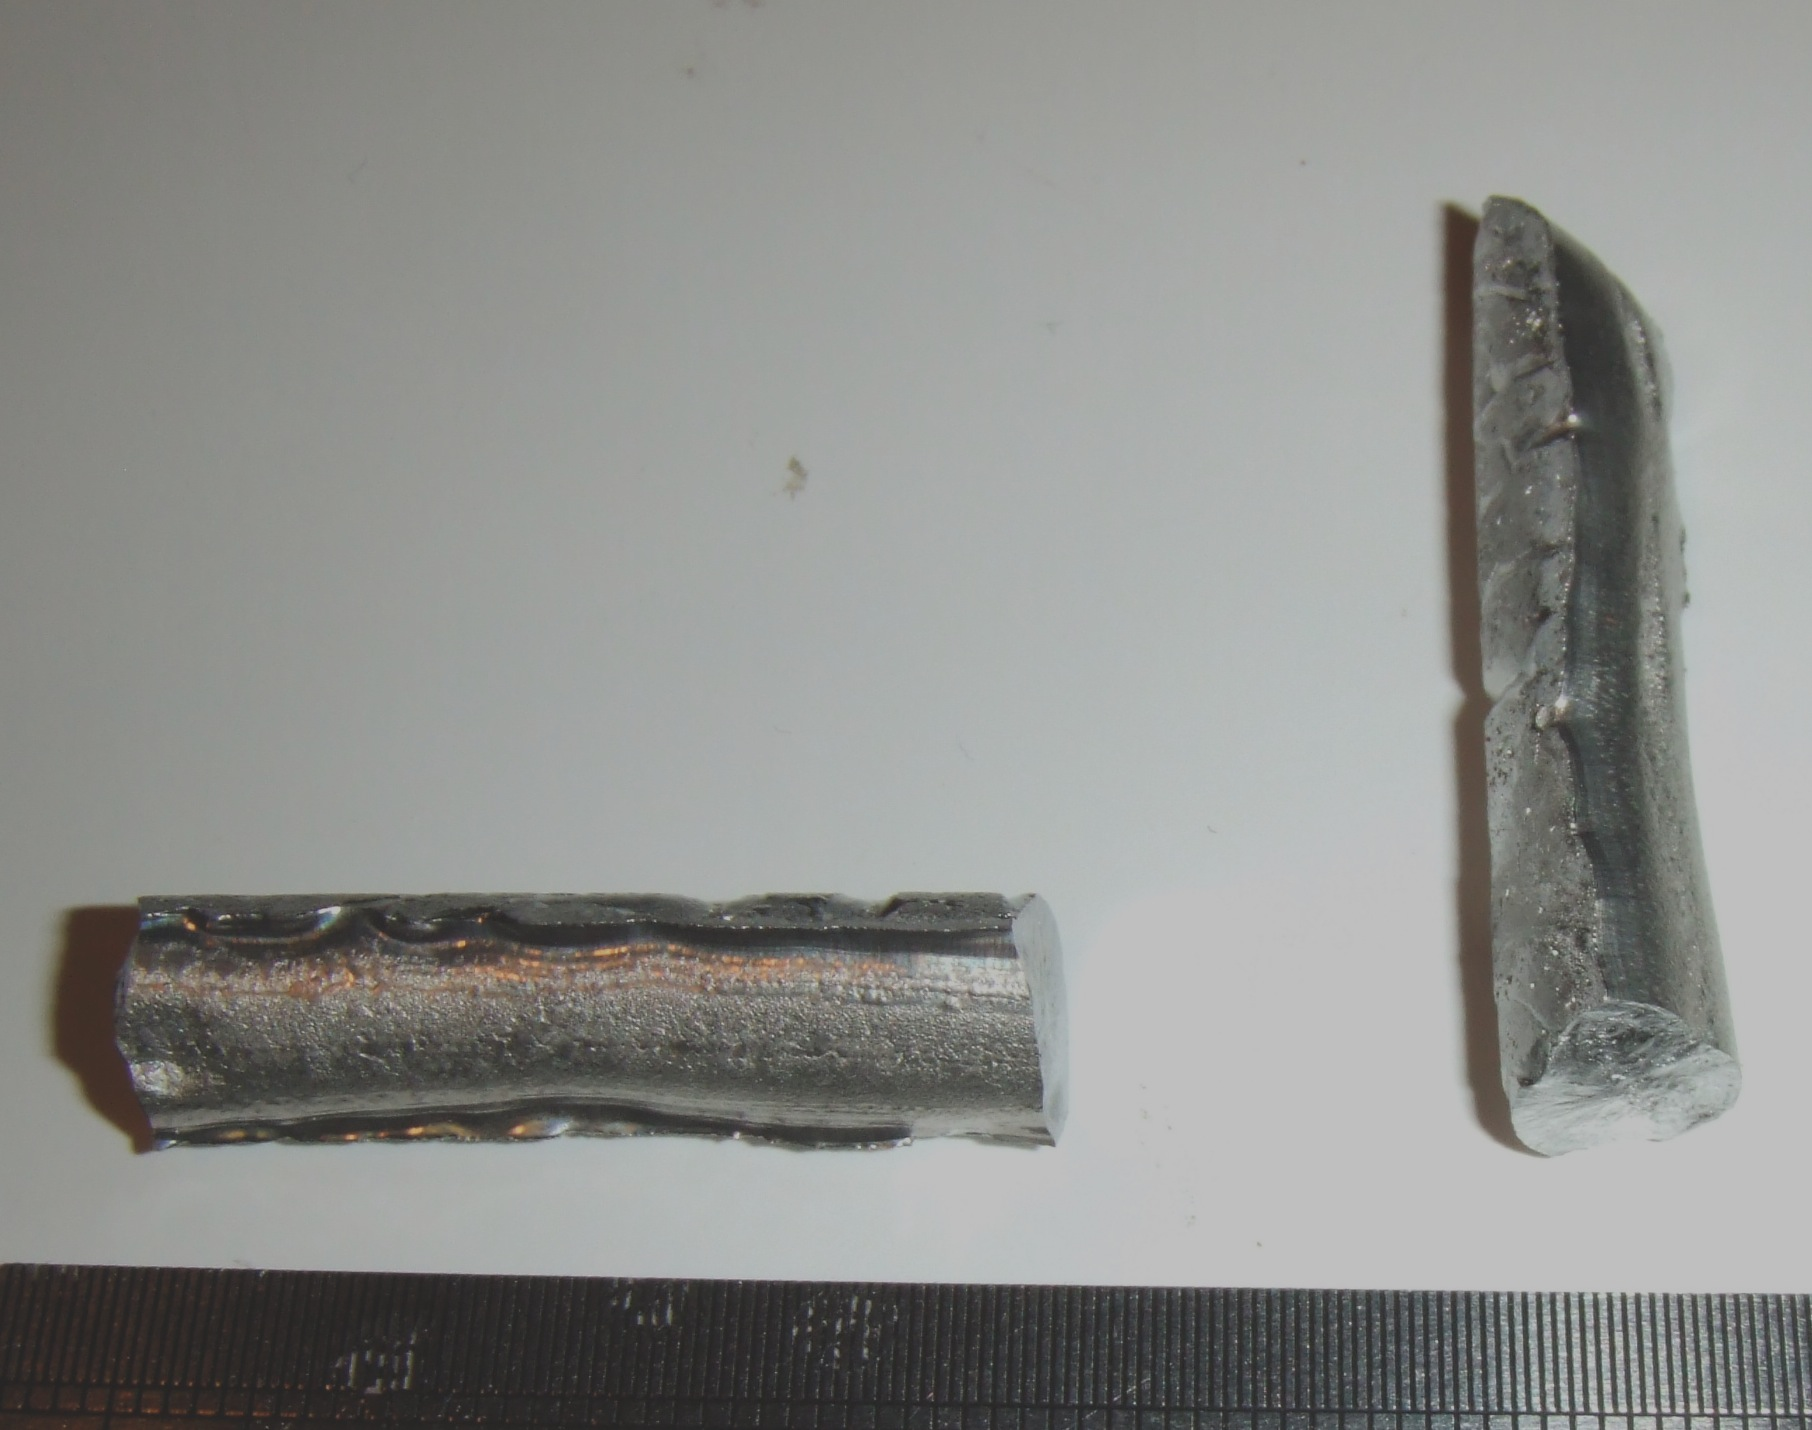
\includegraphics[width=8cm]{crarc}
\caption{Photograph of a typical ingot manufactured by arc-melting that had cracked when cooled from manufacture temperature.}
\label{fig:crarc}
\end{center}
\end{figure}
%
It was thought that the vacuum system of the in-house arc-melt facilities may not be sufficient to prevent nitrogen-embrittlement of the ingots, which may contribute to the crack sensitivity.  There is no quick method to determine whether this was the case.  Manufacturing methods that produce higher ingot quality had to be explored. 

There is a National Laboratory with arc-melt manufacturing facilities located at Department of Materials Science at the University of Birmingham.  Compositions were sent in to Dr.  S. Koohpayeh at the facility to see if purer or more homogeneous samples can be achieved.  Due to the high viscosity of the material, smaller ingots weighing about 5-10 \gram\ were made.  The ingots manufactured had thinner cross-sections than alloys manufactured in-house at the University of Cambridge (Figure \ref{fig:bhamarc}).  This is probably due to higher temperatures achieved during manufacture, which allowed the alloy melt to flow quite well and would therefore result in better mixing.  Several batches of eutecitic alloys were made up, and had their microstructures examined.

%
\begin{figure}[H]
\begin{center}
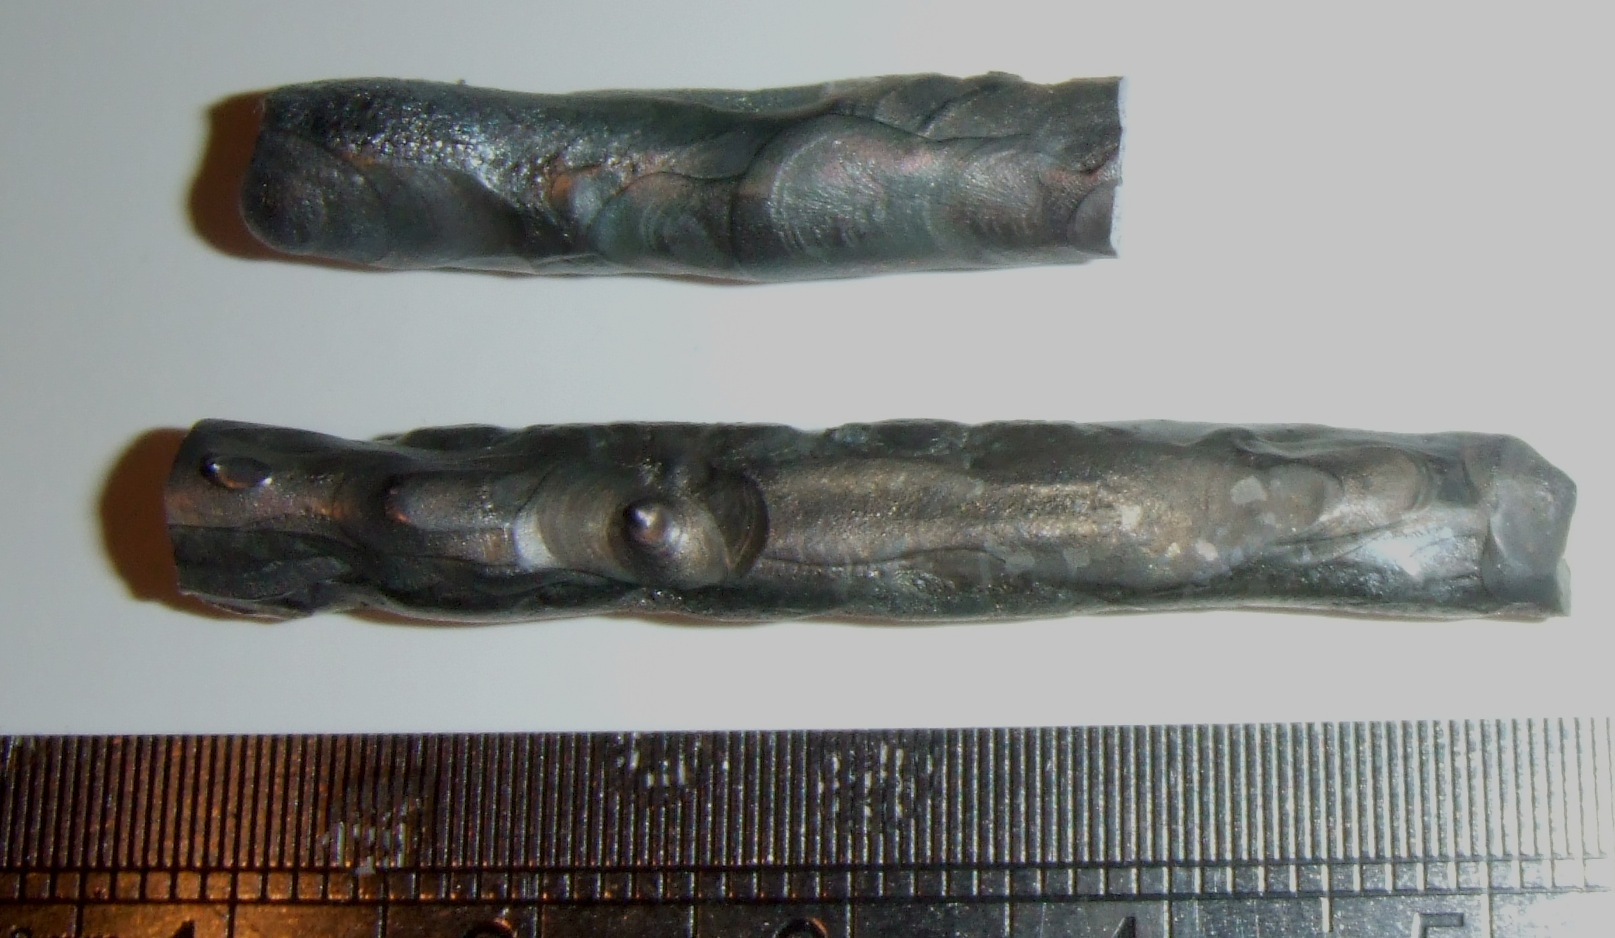
\includegraphics[width=8cm]{bhamarc}
\caption{Photograph of an ingot manufactured by the arc-melt process at the National Laboratory at the University of Birmingham.}
\label{fig:bhamarc}
\end{center}
\end{figure}
%


\subsection{Radio Frequency Solidification Manufacture}

Radio Frequency ingot manufacture using a horizontal cold crucible was tried.  The chromium and silicon coupled very poorly with the RF field.  This meant that not all the feedstock melted.  The melt had very high surface tension, and would bead up.  Also, the vapour pressure of chromium was very high, and a substantial amount of chromium evaporated and condensed onto the inside surface of the water-chilled glass tube.  This meant that the resultant ingot composition would not be particularly close to the nominal composition.

The RF facilities of the Department of Physics, Cambridge, were used as an alternative to in-house alloy manufacture.  Identical manufacturing issues were encountered: incomplete melting of feed ingots, extensive vapourisation of chromium, poor coupling of feedstock and the RF field, and sample cracking during cooling from solidification temperatures (Figure \ref{fig:physicsrf}). 

%
\begin{figure}[H]
\begin{center}
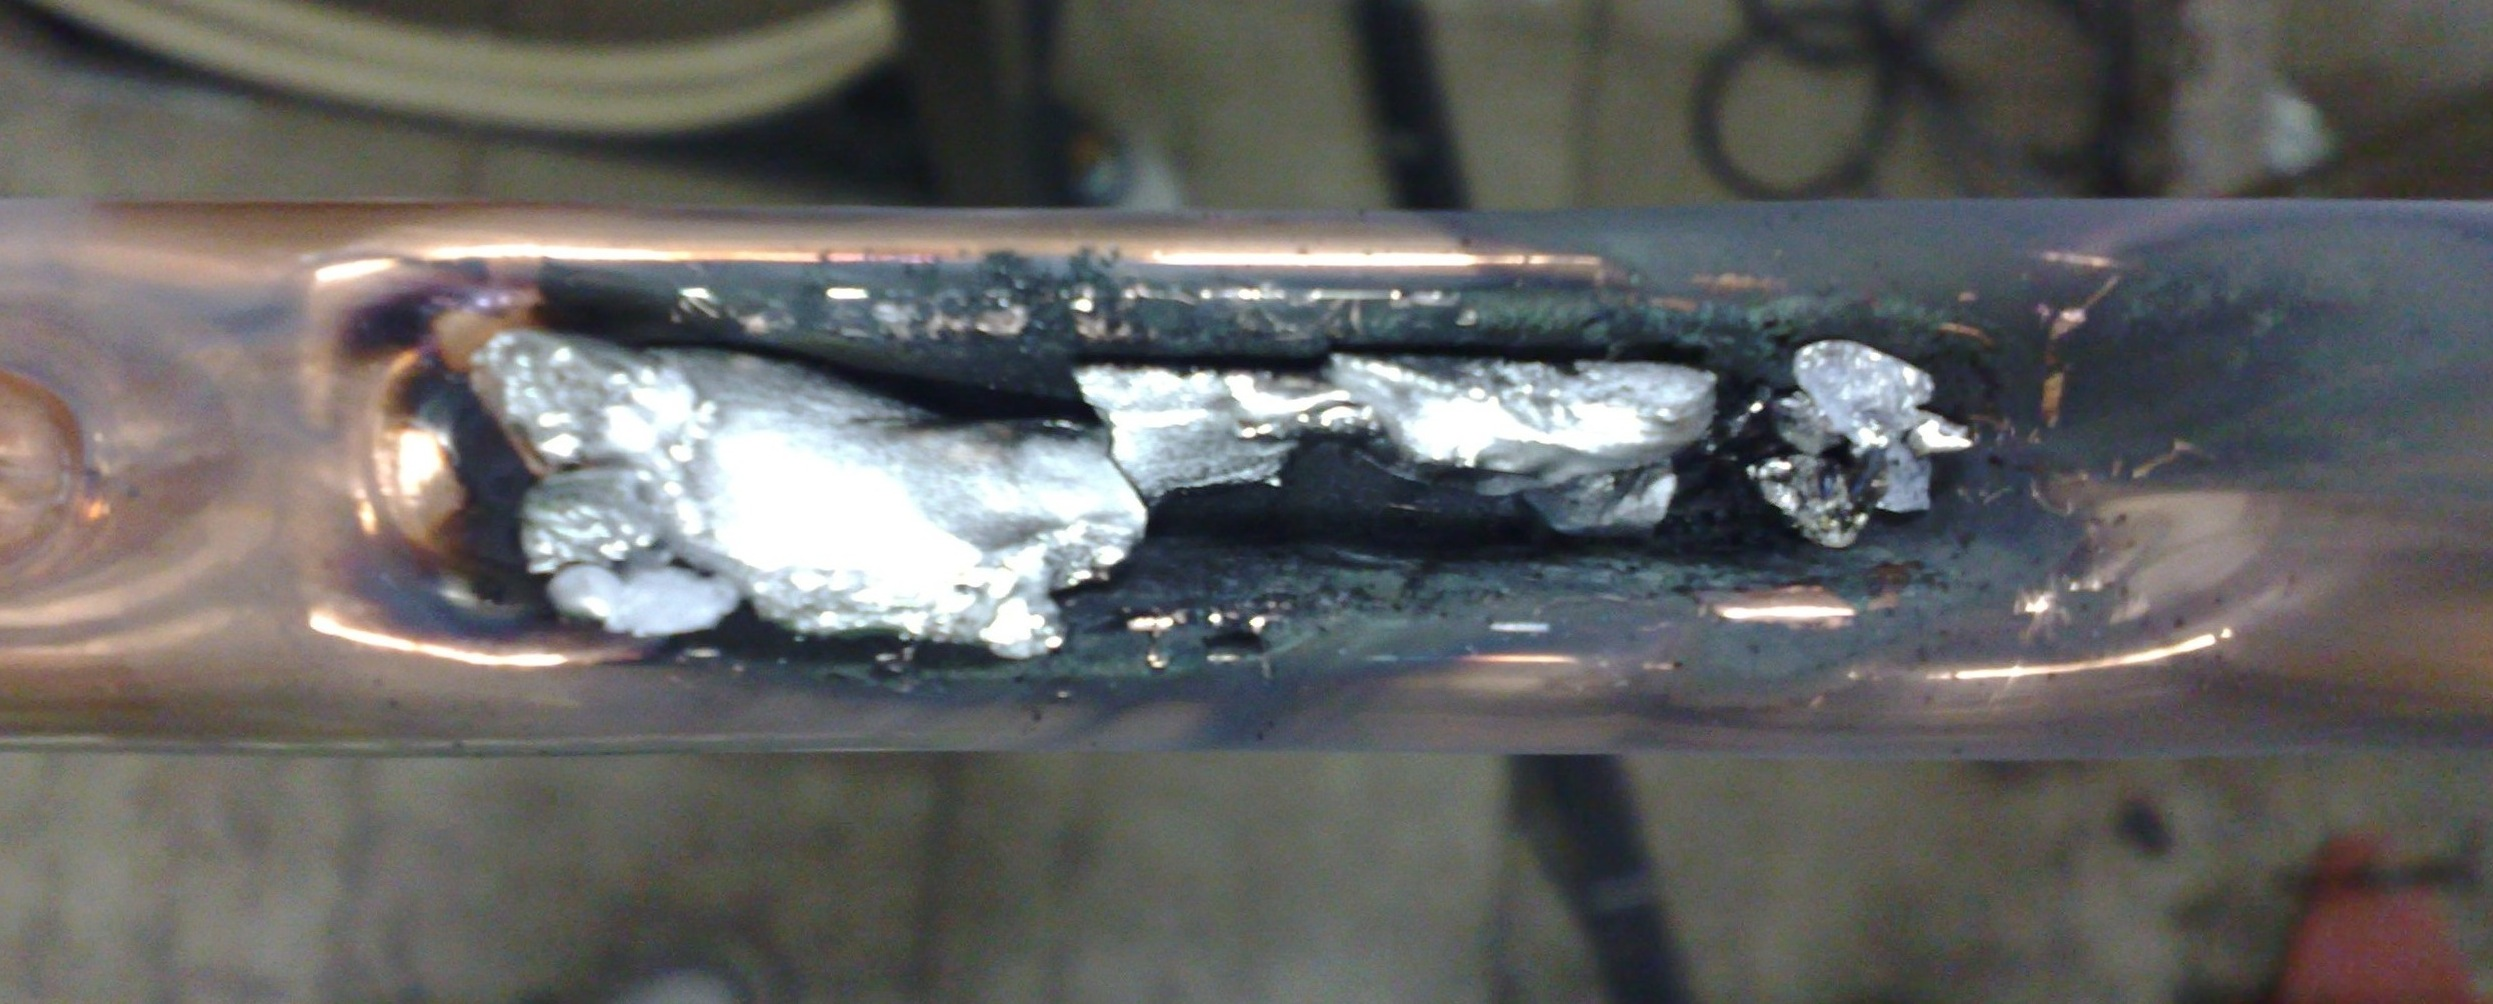
\includegraphics[width=8cm]{physicsrf}
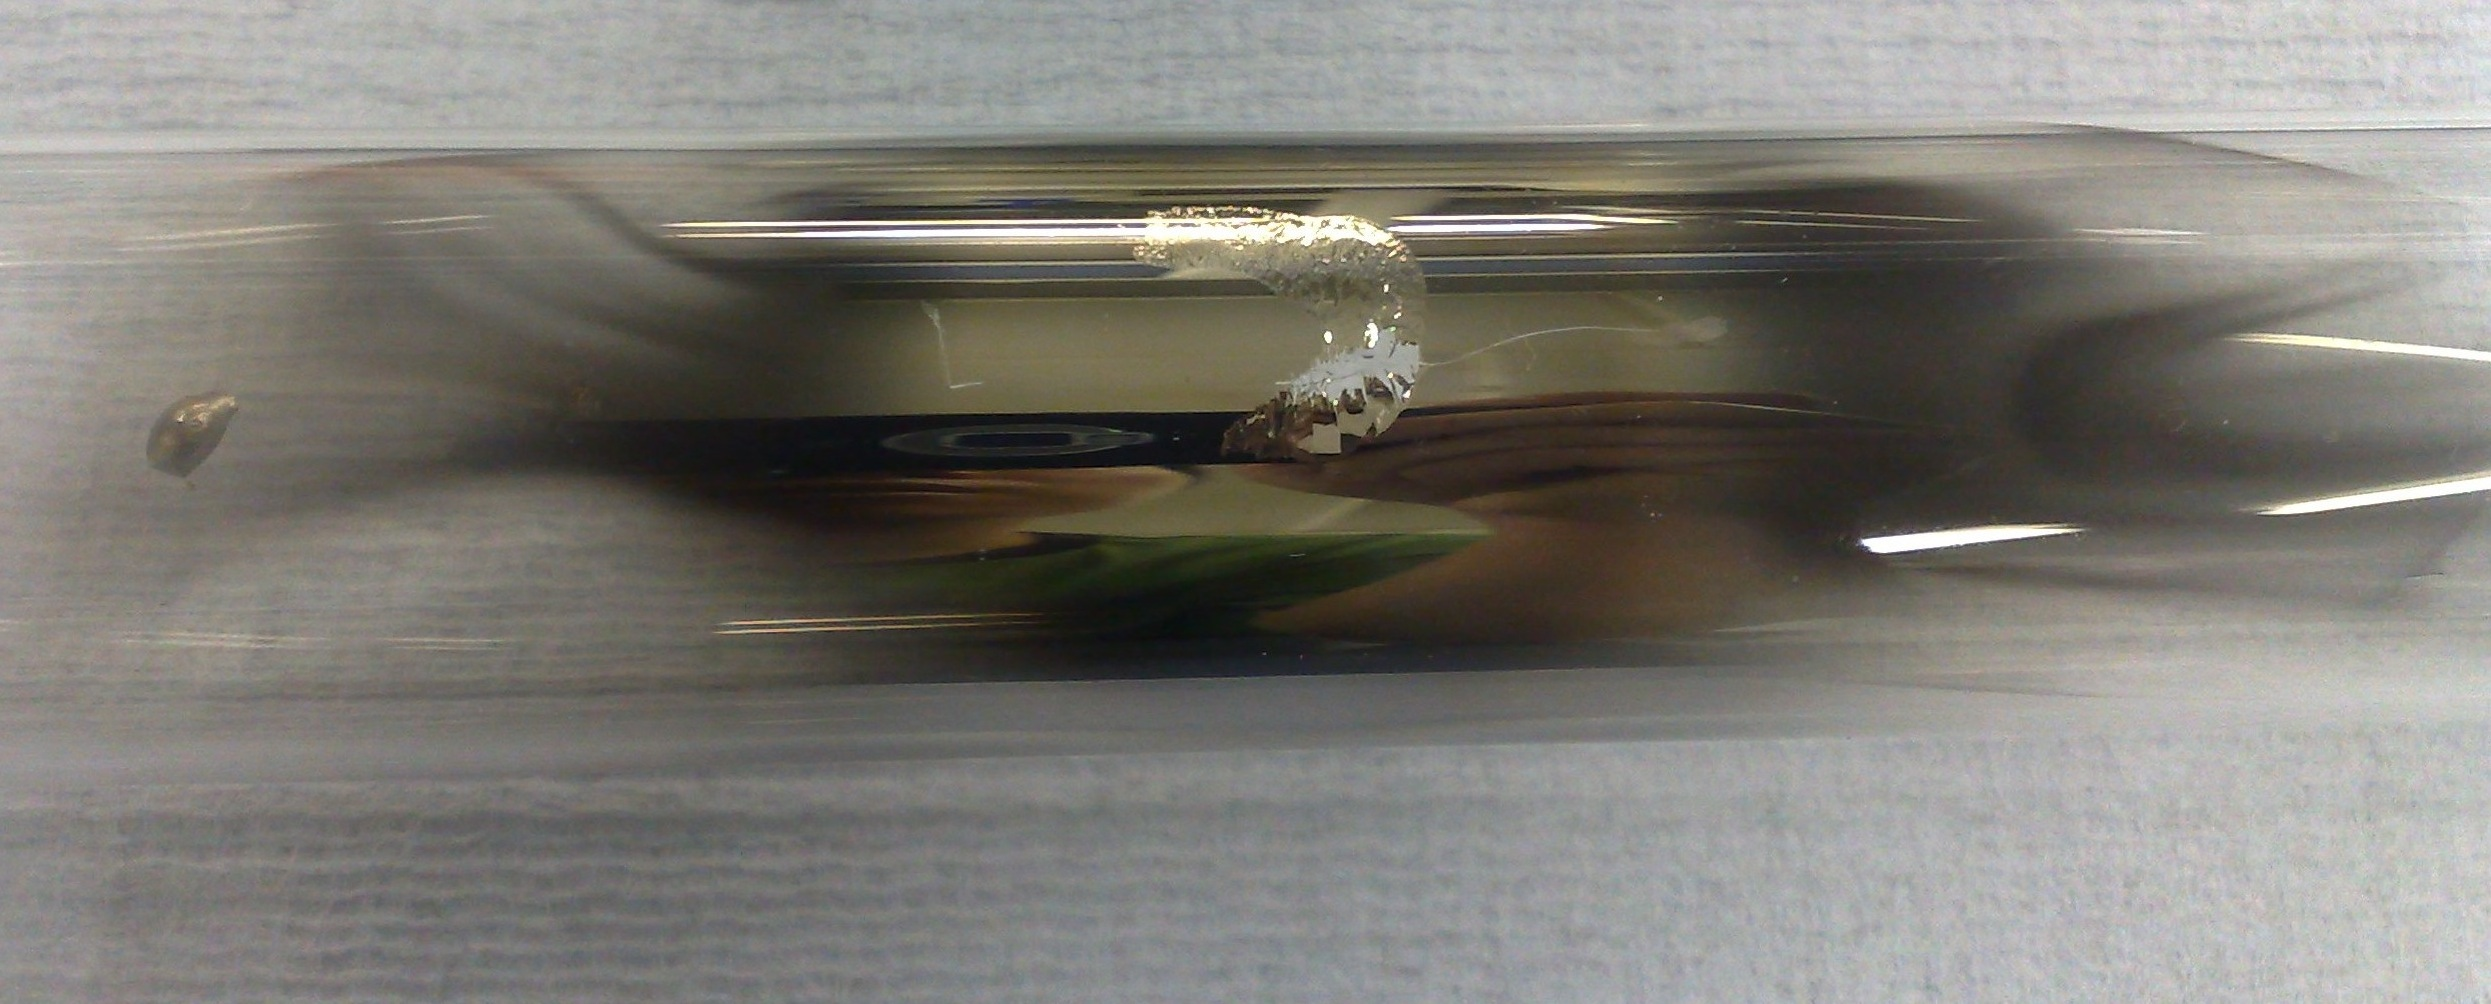
\includegraphics[width=8cm]{physicsrfii}
\caption{Photographs of a Cr--Cr$_3$Si arc-melt ingot that was melted in the horizontal RF furnace at the Department of Physics, Cambridge, and of the quartz receptacle that housed the ingot.}
\label{fig:physicsrf}
\end{center}
\end{figure}
%

\subsection{Graphite Furnace Manufacture}

Melting of alloys in a graphite furnace was attempted.  The graphite Astro$^{\textregistered}$ furnace used was built by Professor Bill Clegg, and can reach temperatures of up to 2400\celsius\ under vaccuum or in an inert atmosphere.  The intention was to cast homogeneous samples with equiaxed grains by bringing all of the feedstock substantially past its melting point to enable proper mixing, and cooling it down slowly so as to minimise the build up of residual stresses which may compromise the ingot's mechanical properties.  

A graphite pot of height 180\milli\metre\ and diameter 100\milli\metre\ was custom-made as a containment vessel in the furnace to contain the feedstock (Figure \ref{fig:cleanpot}).  Its interior surface was sprayed with a coating of boron nitride powder before every cast.  A notch was made into the lip of the pot to prevent its lid from being thrown off in the event of vigorous alloy volatilisation.  A boron nitride crucible with a very thin wall was custom-made to sit snugly inside this graphite pot.  Within this, crucibles of alumina and zirconia were used to hold the feed-stock.  In the event that a reaction were to occur between the alumina or zirconia crucible with the feedstock or melt, this would result in a failure of the crucibles to contain the melt.  Both the graphite pot and boron nitride layer would be in place to react with and contain the feedstock.  This protected the furnace from damage.

%
\begin{figure}[H]
\begin{center}
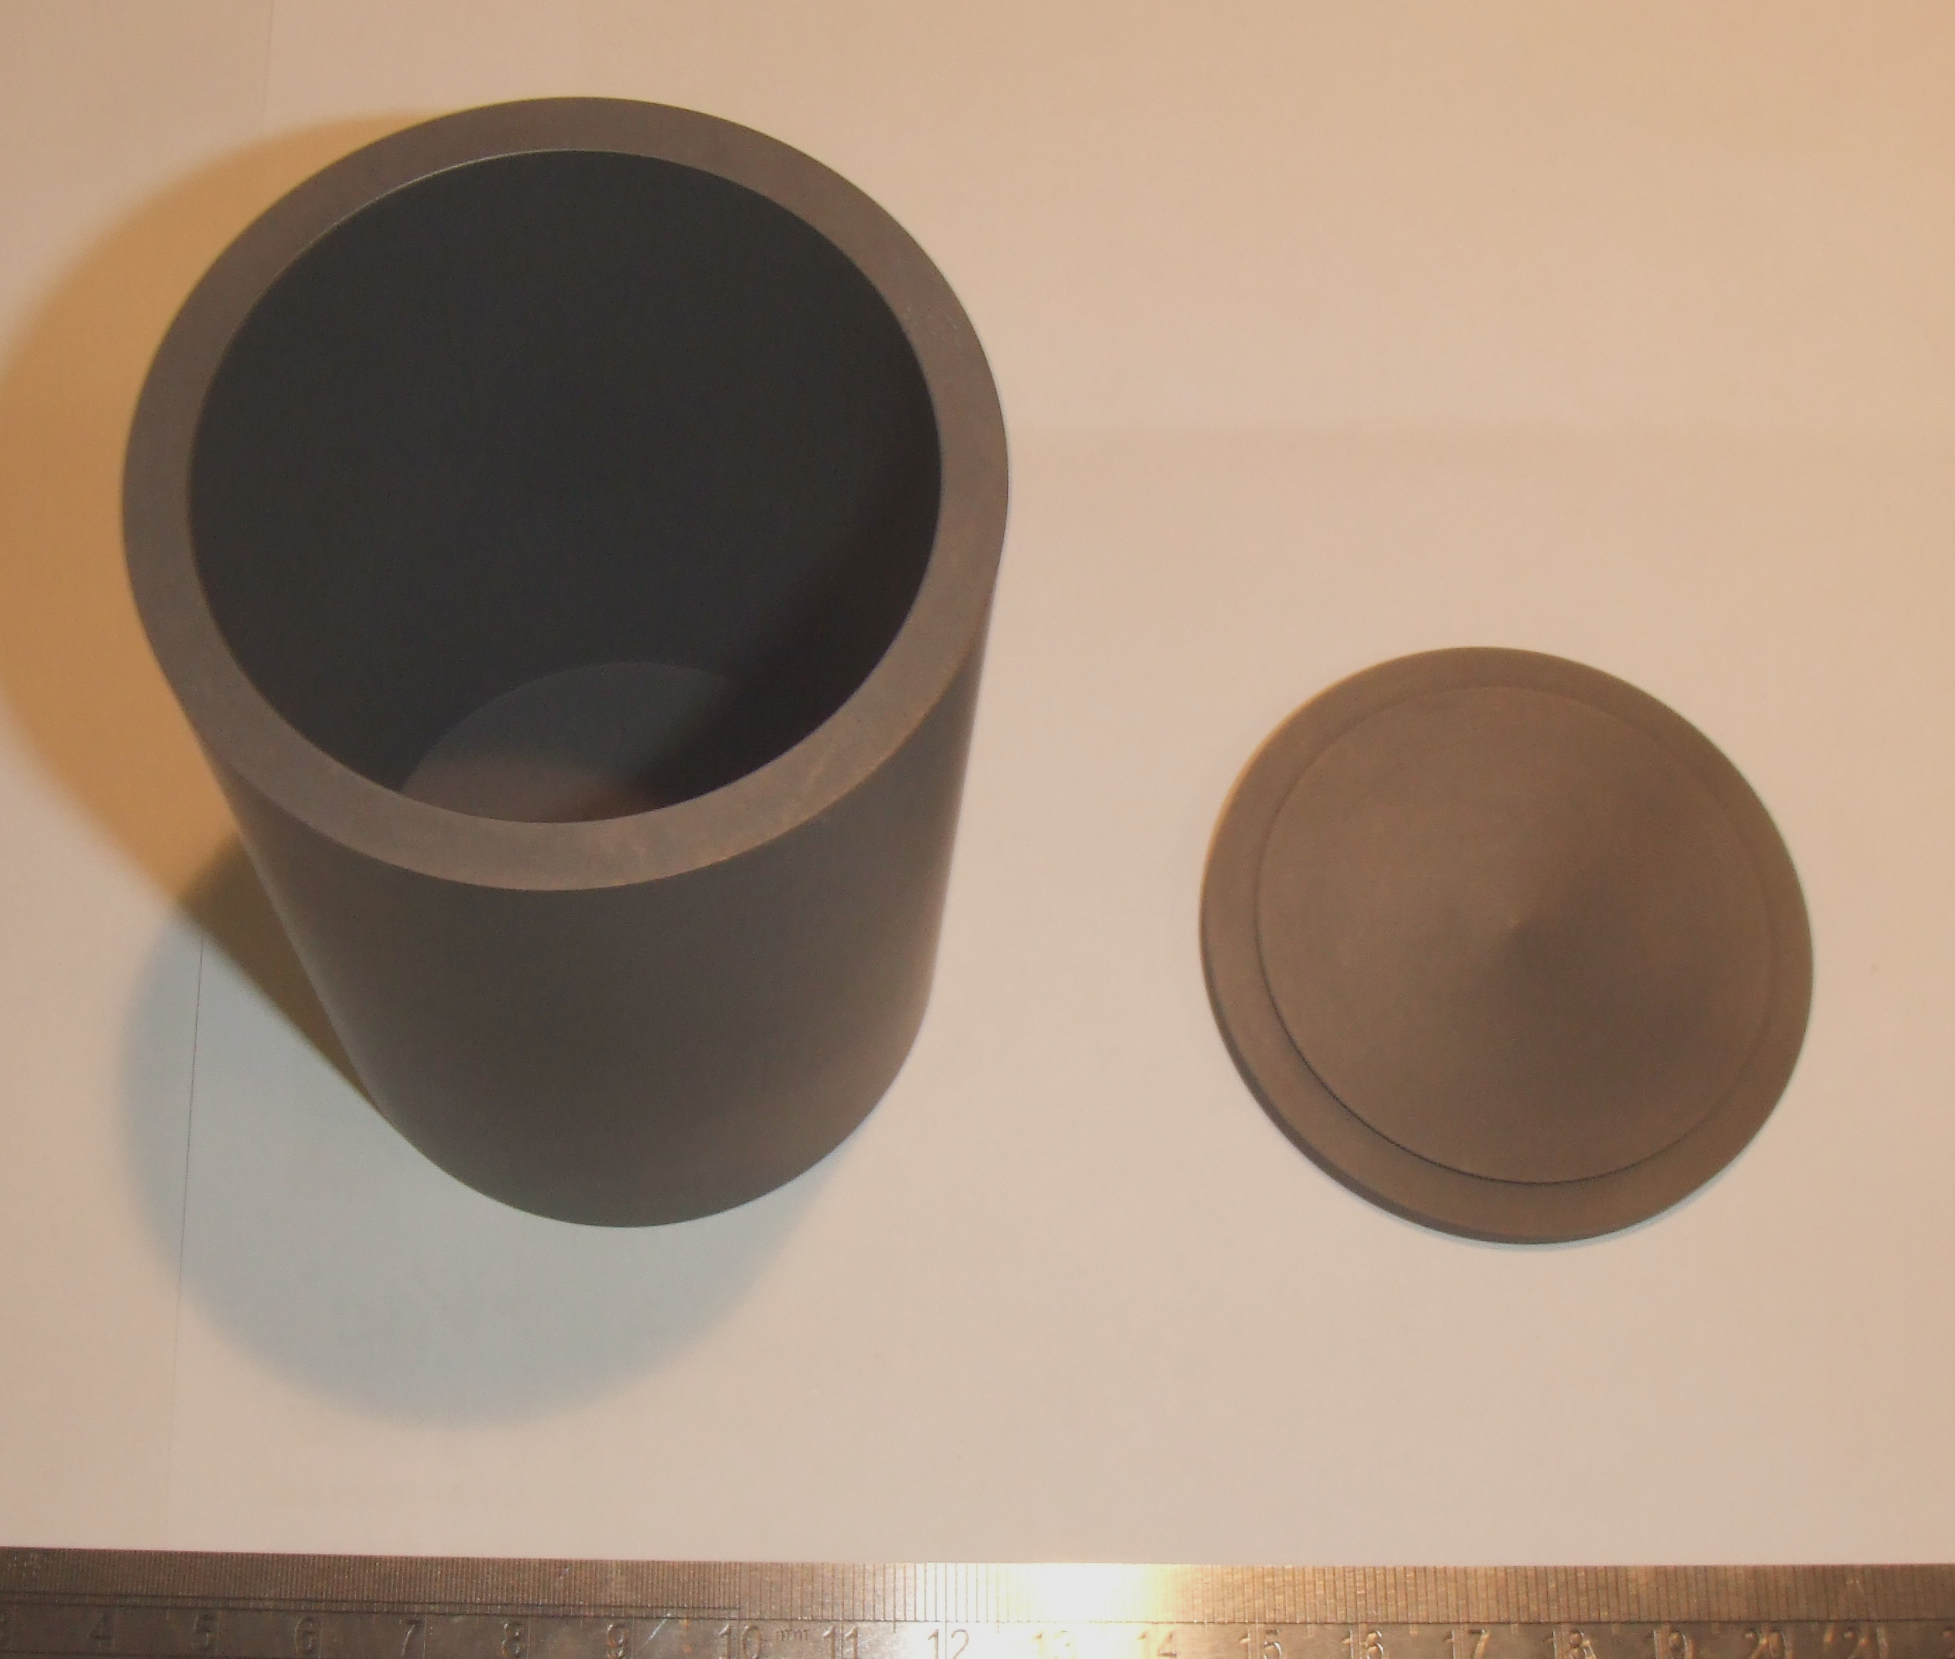
\includegraphics[width=7cm]{cleanpot}
\caption{Photograph of the graphite pot used as a containment vessel in the Astro$^{\textregistered}$ furnace.}
\label{fig:cleanpot}
\end{center}
\end{figure}
%

Arc-melt manufactured ingots were used as feed stock initially.  Cr--Cr$_3$Si was melted to determine its compatibility with alumina crucibles.  Alumina crucibles are relatively cheap, and maintain their integrity up to temperatures of about 1800\celsius, upon which softening occurs.  For runs that would experience temperatures of 1780\celsius\ or higher, zirconia crucibles would be appropriate.  Alloy-crucible compatibility would have to be established. 

The first run had a ramp of 20\celsius/minute to 1735\celsius, a temperature that is 20\celsius\ higher than the feed's theoretical eutectic temperature.  Only partial melting was achieved.  Perhaps the hot zone was not large enough to cause complete melting.  The large graphite pot may be acting as a shield against the radiative heating of the furnace.  Pots used to contain samples are generally thinner-walled and substantially smaller.  A run with the maximum temperature of 1760\celsius\ was set to see if complete melting could be acheived.  The resultant ingot was found to take the shape of the alumina crucible; however, two unmelted pieces of feed were found within the ingot.  Some porosity was seen, and many macro-pores were present, especially when melted in test-tube shaped crucibles (Figure \ref{fig:sponge}).  The melt was either too viscous to take on the shape of the alumina crucible, or was producing vapour that did not manage to escape due to the lack of a mechanism of stirring.  On the whole, also sample dimensions were uneven and small, the cast samples seemed to possess sufficient fracture-toughness.  This is probably due to the very slow cool through the DBTT of the alloy of about 20\celsius/minute, and shows higher sample quality than those produced by arc-melt manufacture.

%
\begin{figure}[H]
\begin{center}
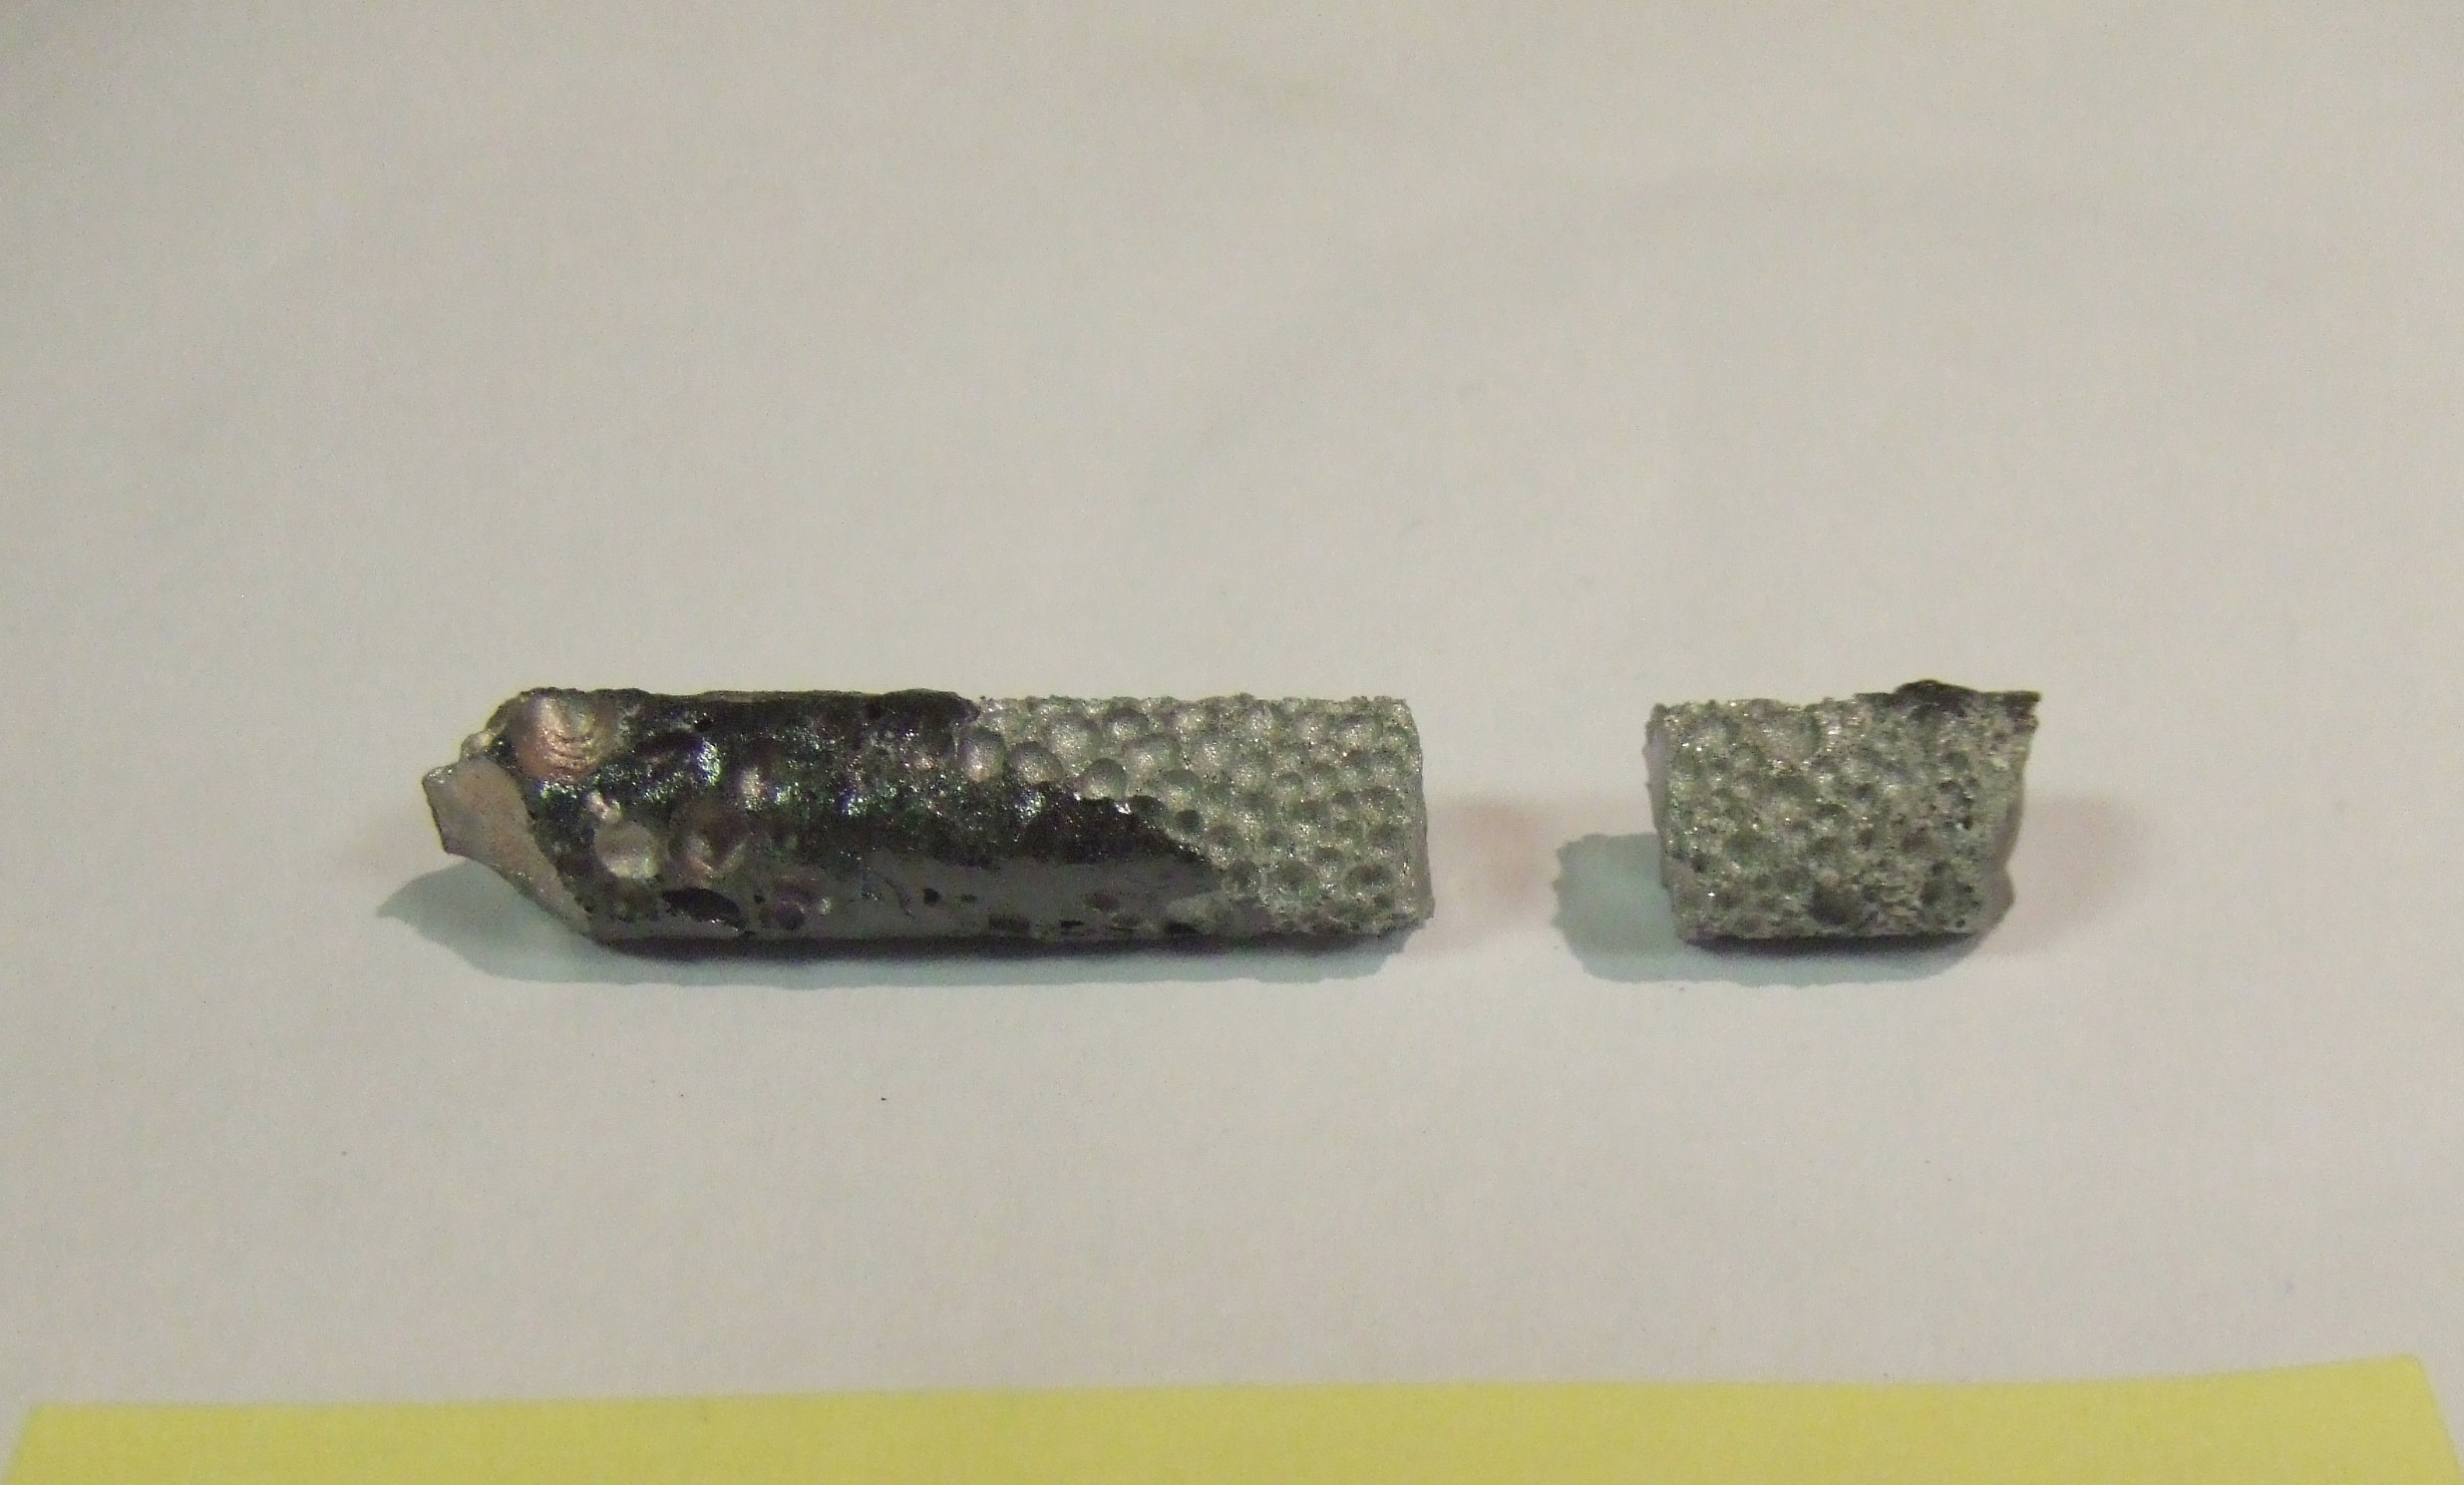
\includegraphics[width=9cm]{spongei}
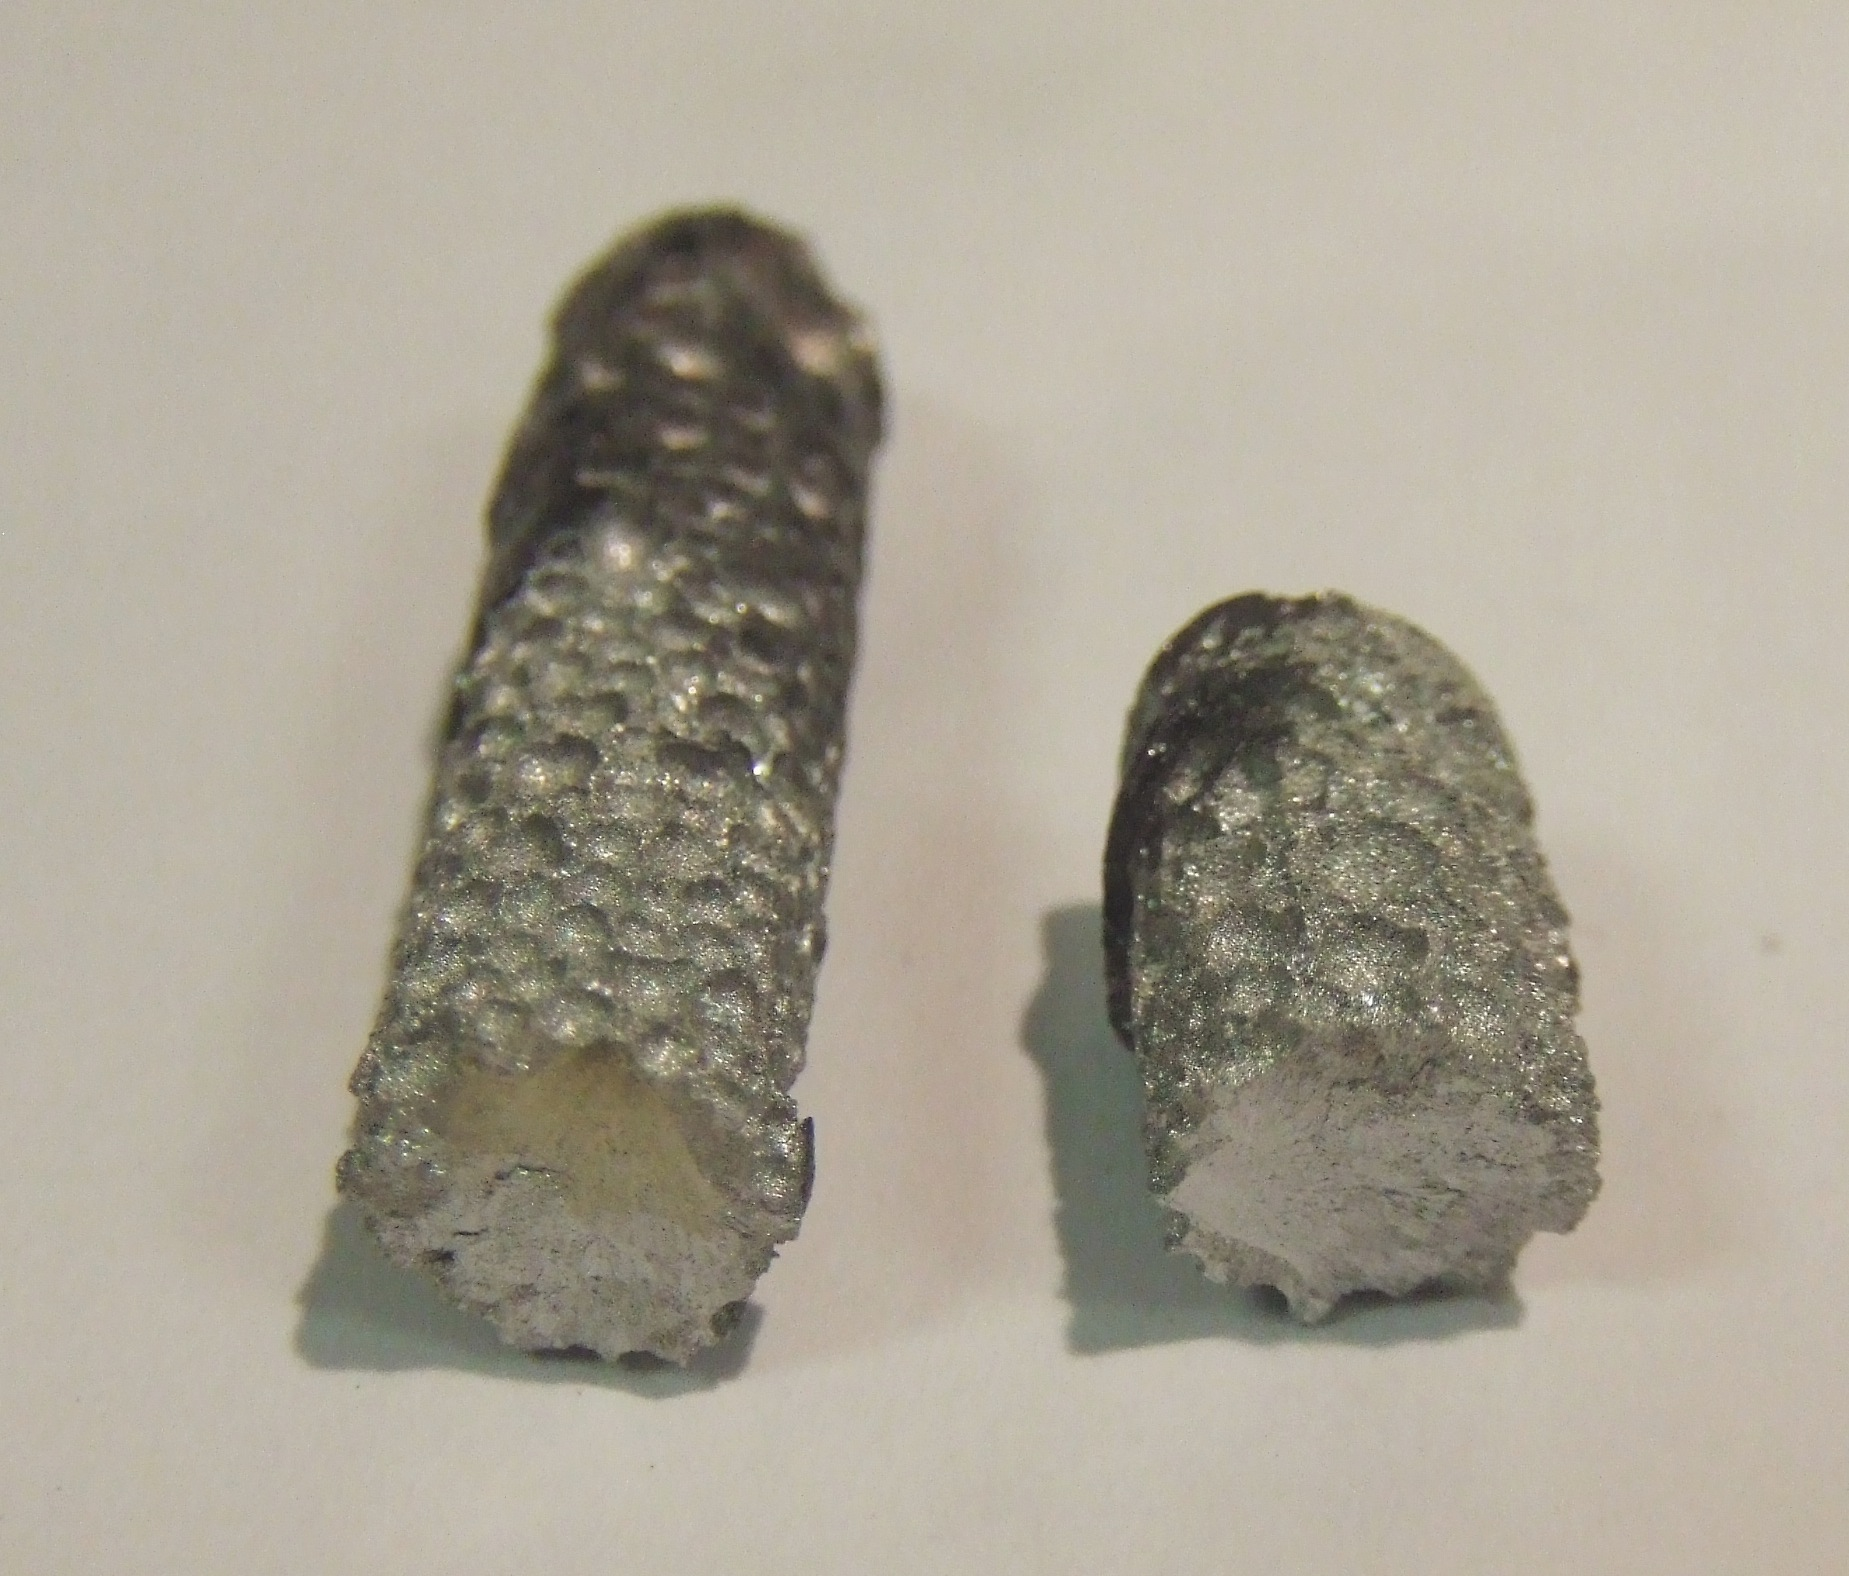
\includegraphics[width=6.36cm]{spongeii}
\caption{Photographs of two views of a sample made from arc-melt feedstock in a narrow zirconia crucible placed in the Astro$^{\textregistered}$ furnace.}
\label{fig:sponge}
\end{center}
\end{figure}
%
%
\begin{figure}[H]
\begin{center}
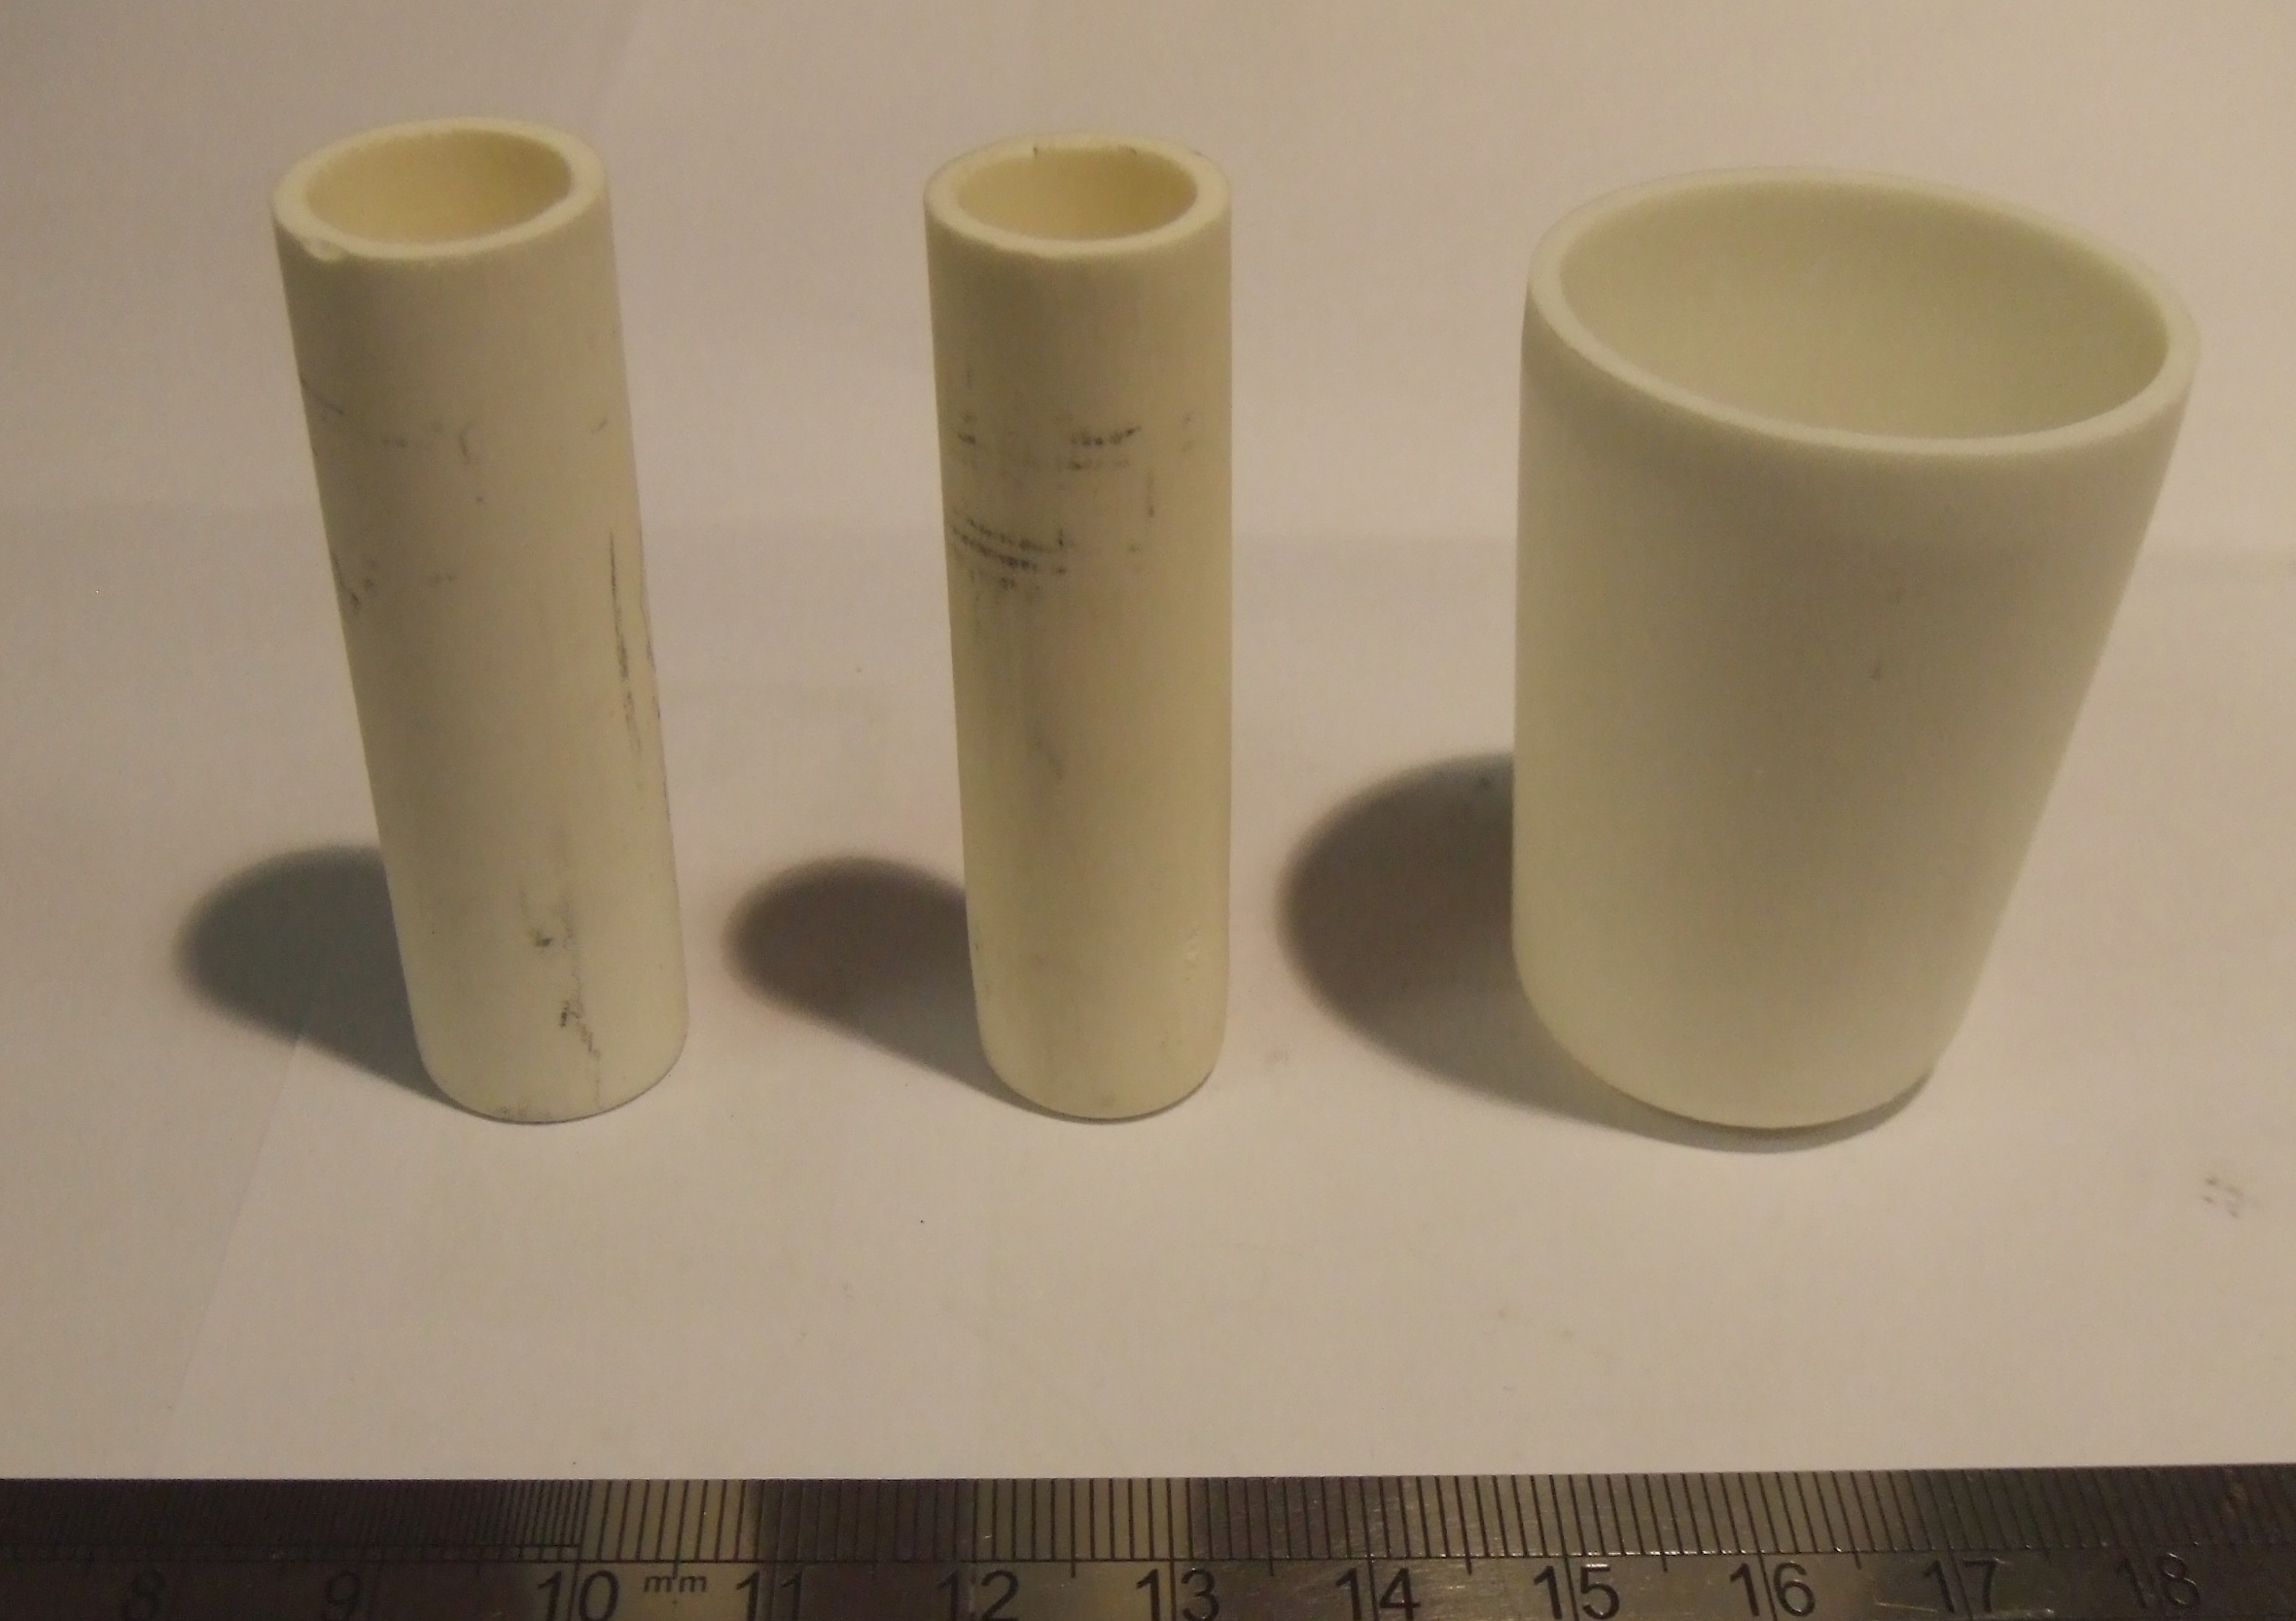
\includegraphics[width=9cm]{squat}
\caption{Photograph of the zirconia crucibles used in alloy manufacture in the Astro$^{\textregistered}$ furnace}
\label{fig:squat}
\end{center}
\end{figure}
%
The dimensions of crucibles used were changed from long, thin test tubes to squat, wide pots.  Squat pots would allow the melt to form into a suitably large and regular ingots more easily by reducing their surface area to volume ratios.  The intention was to produce enough suitable stock to manufacture homogeneous compression test specimens that could then be tested.  Arc-melt manufacture ingots were used as feed in these squat pots, and brought up to 1800\celsius\ at 20\celsius/minute, held for 15 minutes, and cooled at 20\celsius/minute.  This maximum temperature is high enough to melt the Cr$_3$Si intermetallic. Zirconia crucibles were used as they can withstand such high temperatures.  No significant reaction occurred between the ingot and the crucible.  Substantial vapour from the melt was found to have condensed on the inner surface of the graphite pot lid (Figure \ref{fig:dirtypot}a).  As zirconia crucibles are four times more expensive than alumina ones, when the option to use zirconia-coated alumina crucibles at a price that was equivalent to that of an alumina crucible, it was taken.  One such crucible was used for a Cr--Cr$_3$Si ingot, and was found to undergo a reaction  at temperatures under 1800\celsius, either with the feedstock or with itself (Figure \ref{fig:dirtypot}b).  The feedstock mostly evaporated during such conditions, possibly by forming intermediate compounds of lower melting points.

%
\begin{figure}[H]
\begin{center}
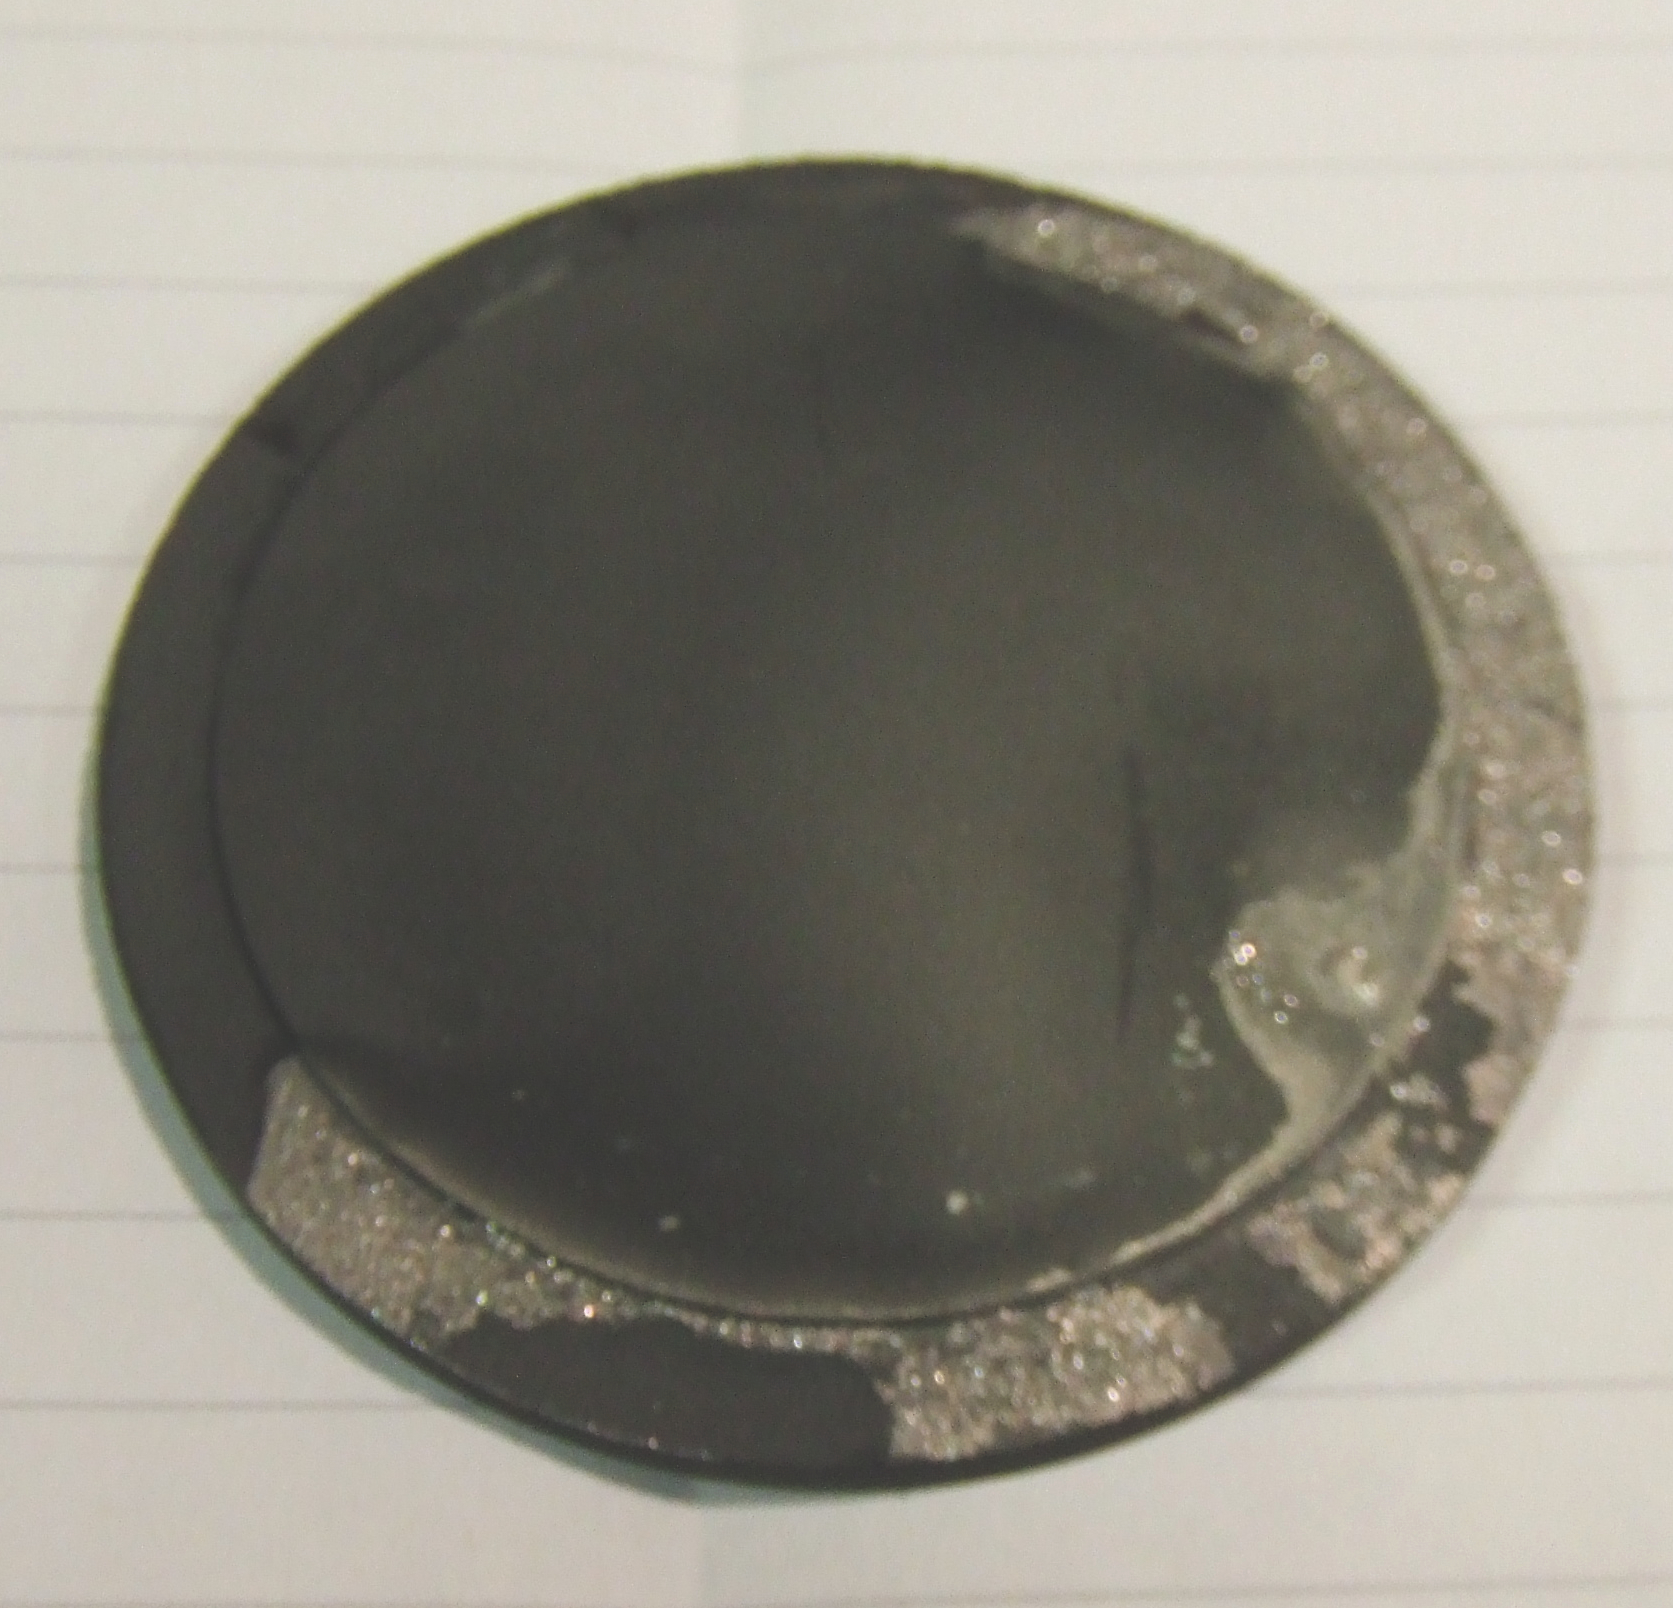
\includegraphics[width=7.8cm]{dirtypotlid}
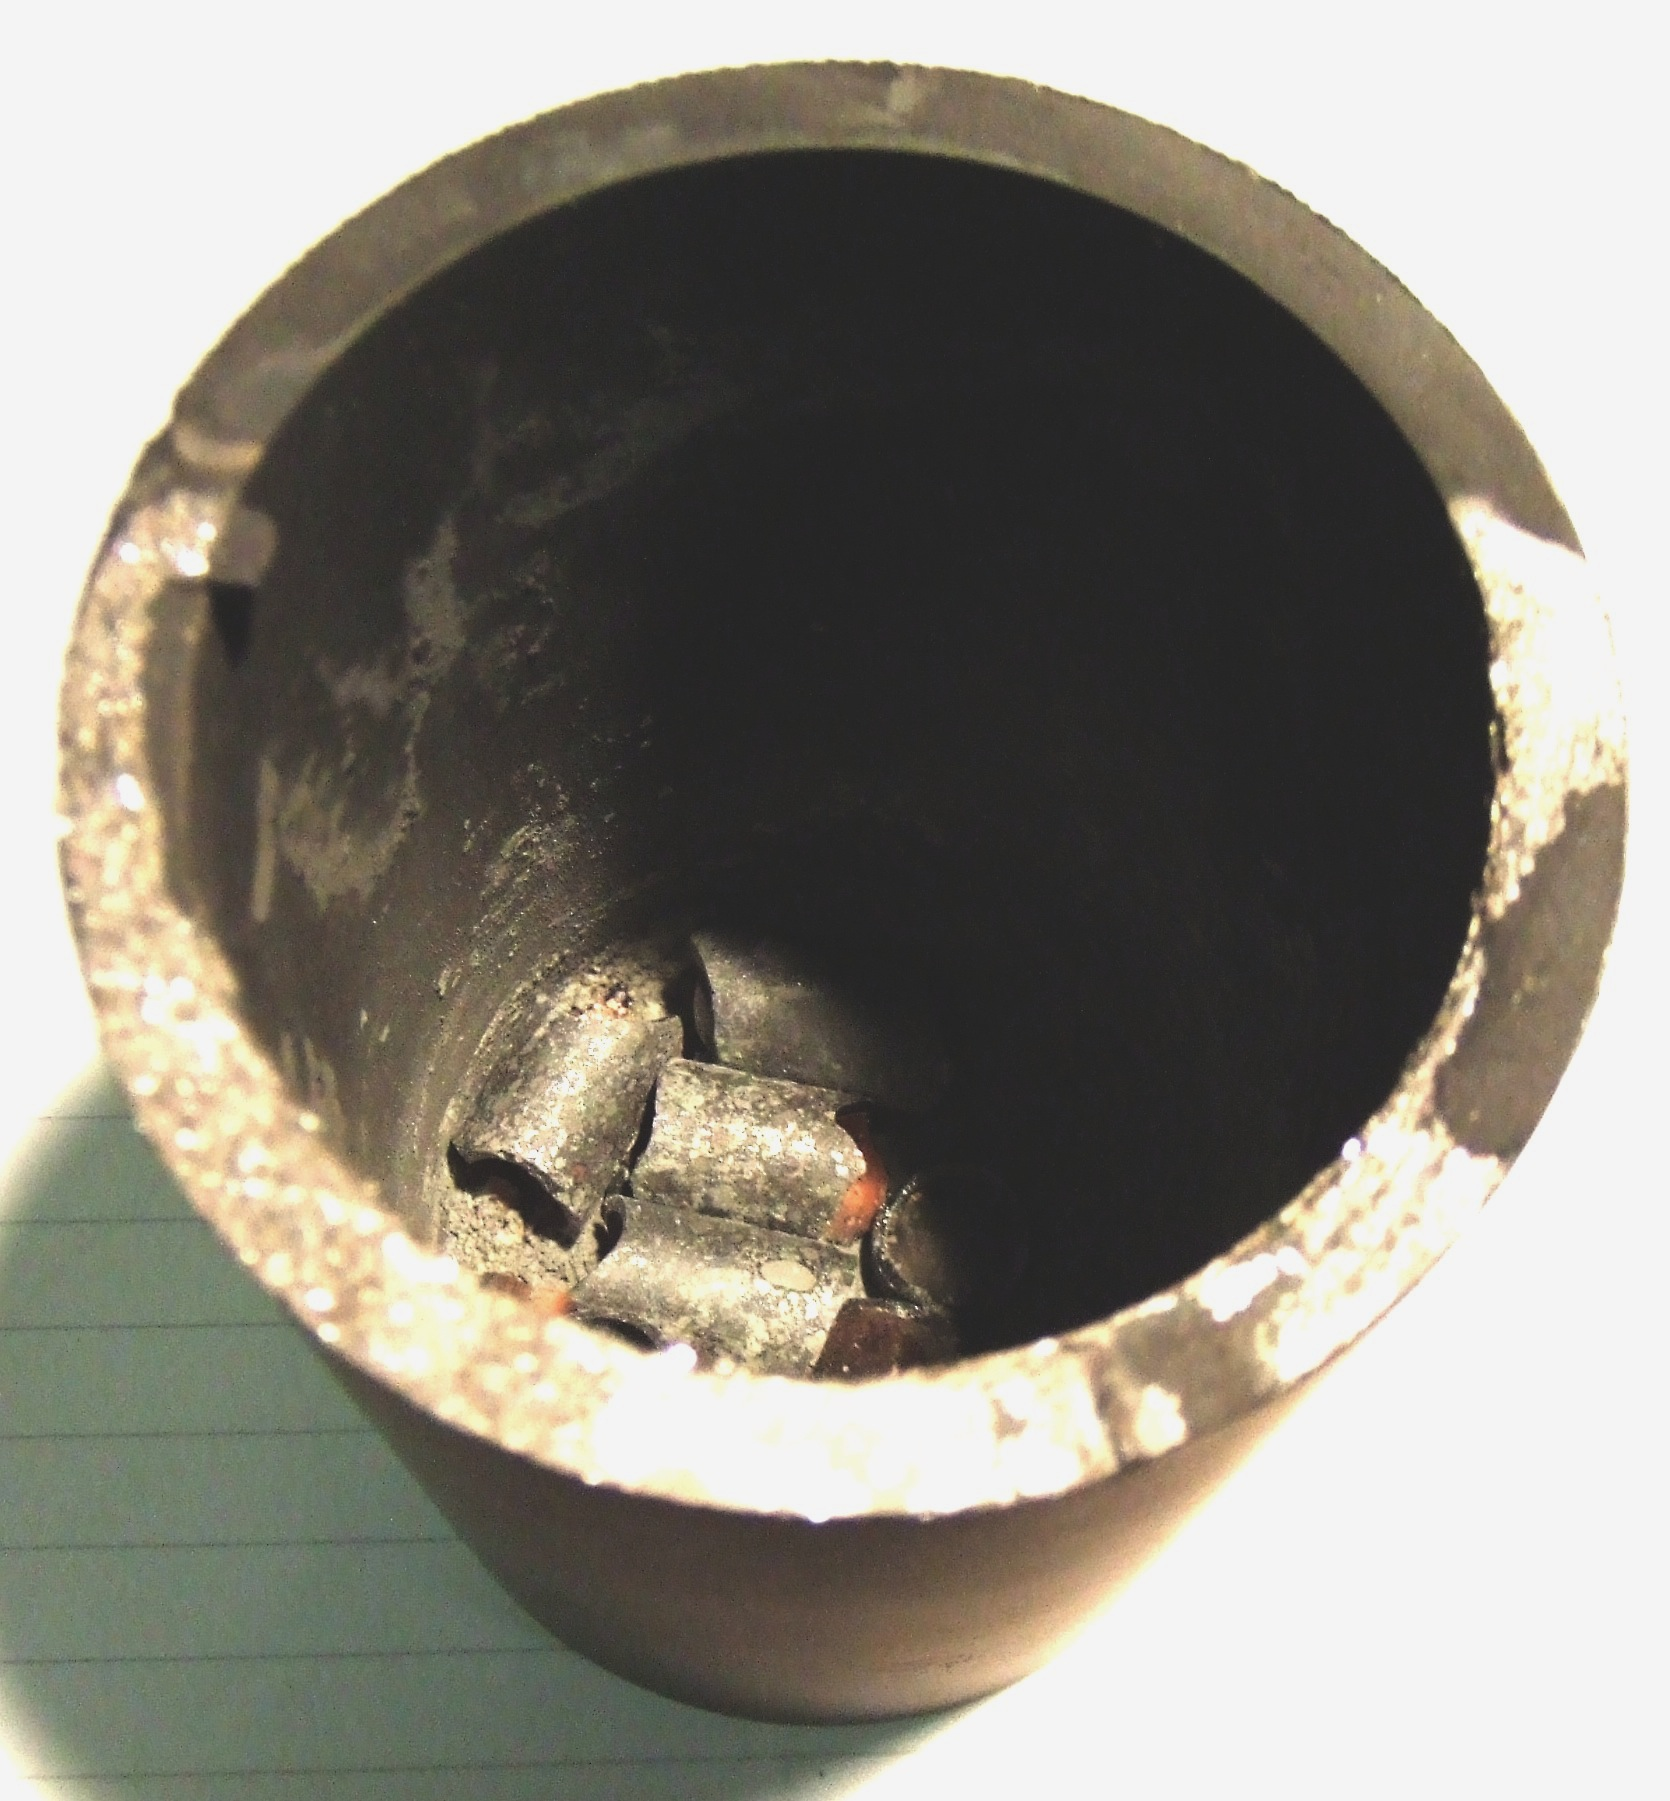
\includegraphics[width=7cm]{dirtypot}
\caption{Photograph of the graphite pot after feedstock reacted with the crucibles in the Astro$^{\textregistered}$ furnace.}
\label{fig:dirtypot}
\end{center}
\end{figure}
%

Fine, granular stock of the alloys' elemental components was also used as feed.  Gaseous Cr that escapes from the melt coalesce and remain on the crucible wall, resulting in a sponge-like final product with some internal porosity.  When this granular feed was cold-pressed into pellets, porosity was slightly reduced, but the resultant ingot integrity was still insufficient.  Segregation due to large differences in element densities was also observed.  Si does not melt completely although it has a much lower melting point than the eutectic (Figure \ref{fig:CrSi}).  This is likely due to poor melt-mixing stemming from the lack of a mixing mechanism. 

All sensible combinations of variables for alloy manufacture have been done under an Ar atmosphere and under vacuum, but none has been successful.  High melt viscosity, the lack of a mechanism for stirring the melt, the differences in Cr and Si volatility, are some of the reasons.  This method was abandoned.


\subsection{Plasma-Melting}

Plasma-melting (PM) was pursued as alternative route of manufacture to arc-melting.  The National Laboratory at the University of Birmingham has a PM facility that can manufacture dome-shaped ingots weighing between 1.0--2.5 \kilogram.  This uses ionised argon gas to melt the feedstock which is contained in a hemispherical water-chilled copper hearth.  As there is no focussed heat-source in PM manufacture, the temperatures experienced by an ingot would be less than temperatures experienced during arc-melt manufacture.  Ideally, this would translate into less volatilisation of feed-stock, and greater homogeniety in the end product.  They are hemi-spherical and the cooling rates on the domed surface of the ingot are in contact with a water-chilled copper hearth, and are estimated to be of the same magnitude experienced by samples during the arc-melt process.  The cooling rates are much lower near the flat surface of the ingot due to the latent heat in the large ingot.  All samples except V$_3$Si exhibited cracking.  The high cooling rate differential experienced by the ingots.  Despite its superiority to the arc-melt method, it was not used as the primary method of alloy feedstock manufacture as there was an extensive waiting period of two years till the first chance to have ingots manufactured arose.

99.95\% purity Cr pellets, Si chips, V pieces, Ta pieces, W pieces, and Al pieces were used as feed.  The ingots weighed between 1.5--2.2 \kilogram, depending on the packing density of the feedstock used.  They were flipped and re-melted another three times each.  Two educated guesses of slightly different compositions were made for each of the binary alloys, in the hope that an ingot of each binary would have mostly lamellar eutectic.  Cr--Cr$_3$Si 15at.\%, Cr--Cr$_3$Si 16at.\%, V--V$_3$Si with 11at.\% Si and V--V$_3$Si with 13at.\% Si.  Then, \ilovewill{山}Ta, \ilovewill{山}TaAl (Figure \ref{fig:pmsantaal}), \ilovewill{山}W and \ilovewill{山}WAl were made.  The ternary eutectics were not manufactured.  This was deemed unneccessary as the arc-melted ingots, despite their inhomogenieties, showed continuous phase fields across both the solid-solution and the X$_3$Si  intermetallic. 

All ingots with the exception of V--V$_3$Si were susceptible to cracking during cooling and machining.  All ingots were cut with electro-discharge spark-machining.  Longitudinal cross-sections of all ingots showed pieces of remnant refractory metal (Ta and W) feedstock that remained unmelted (Figure \ref{fig:pmsantaii}a).  Transverse cross-sections taken near the flat surfaces of the ingots showed fragments of unmelted Si situated in a plane about 1  \centi\metre\ from the flat surfaces (Figure \ref{fig:pmsantaii}b).  The presence of substantial unmelted stock material is possibly be due to the high viscosity and surface tension induced by the high silicon and chromium contents. 



%
\begin{figure}[H]
\begin{center}
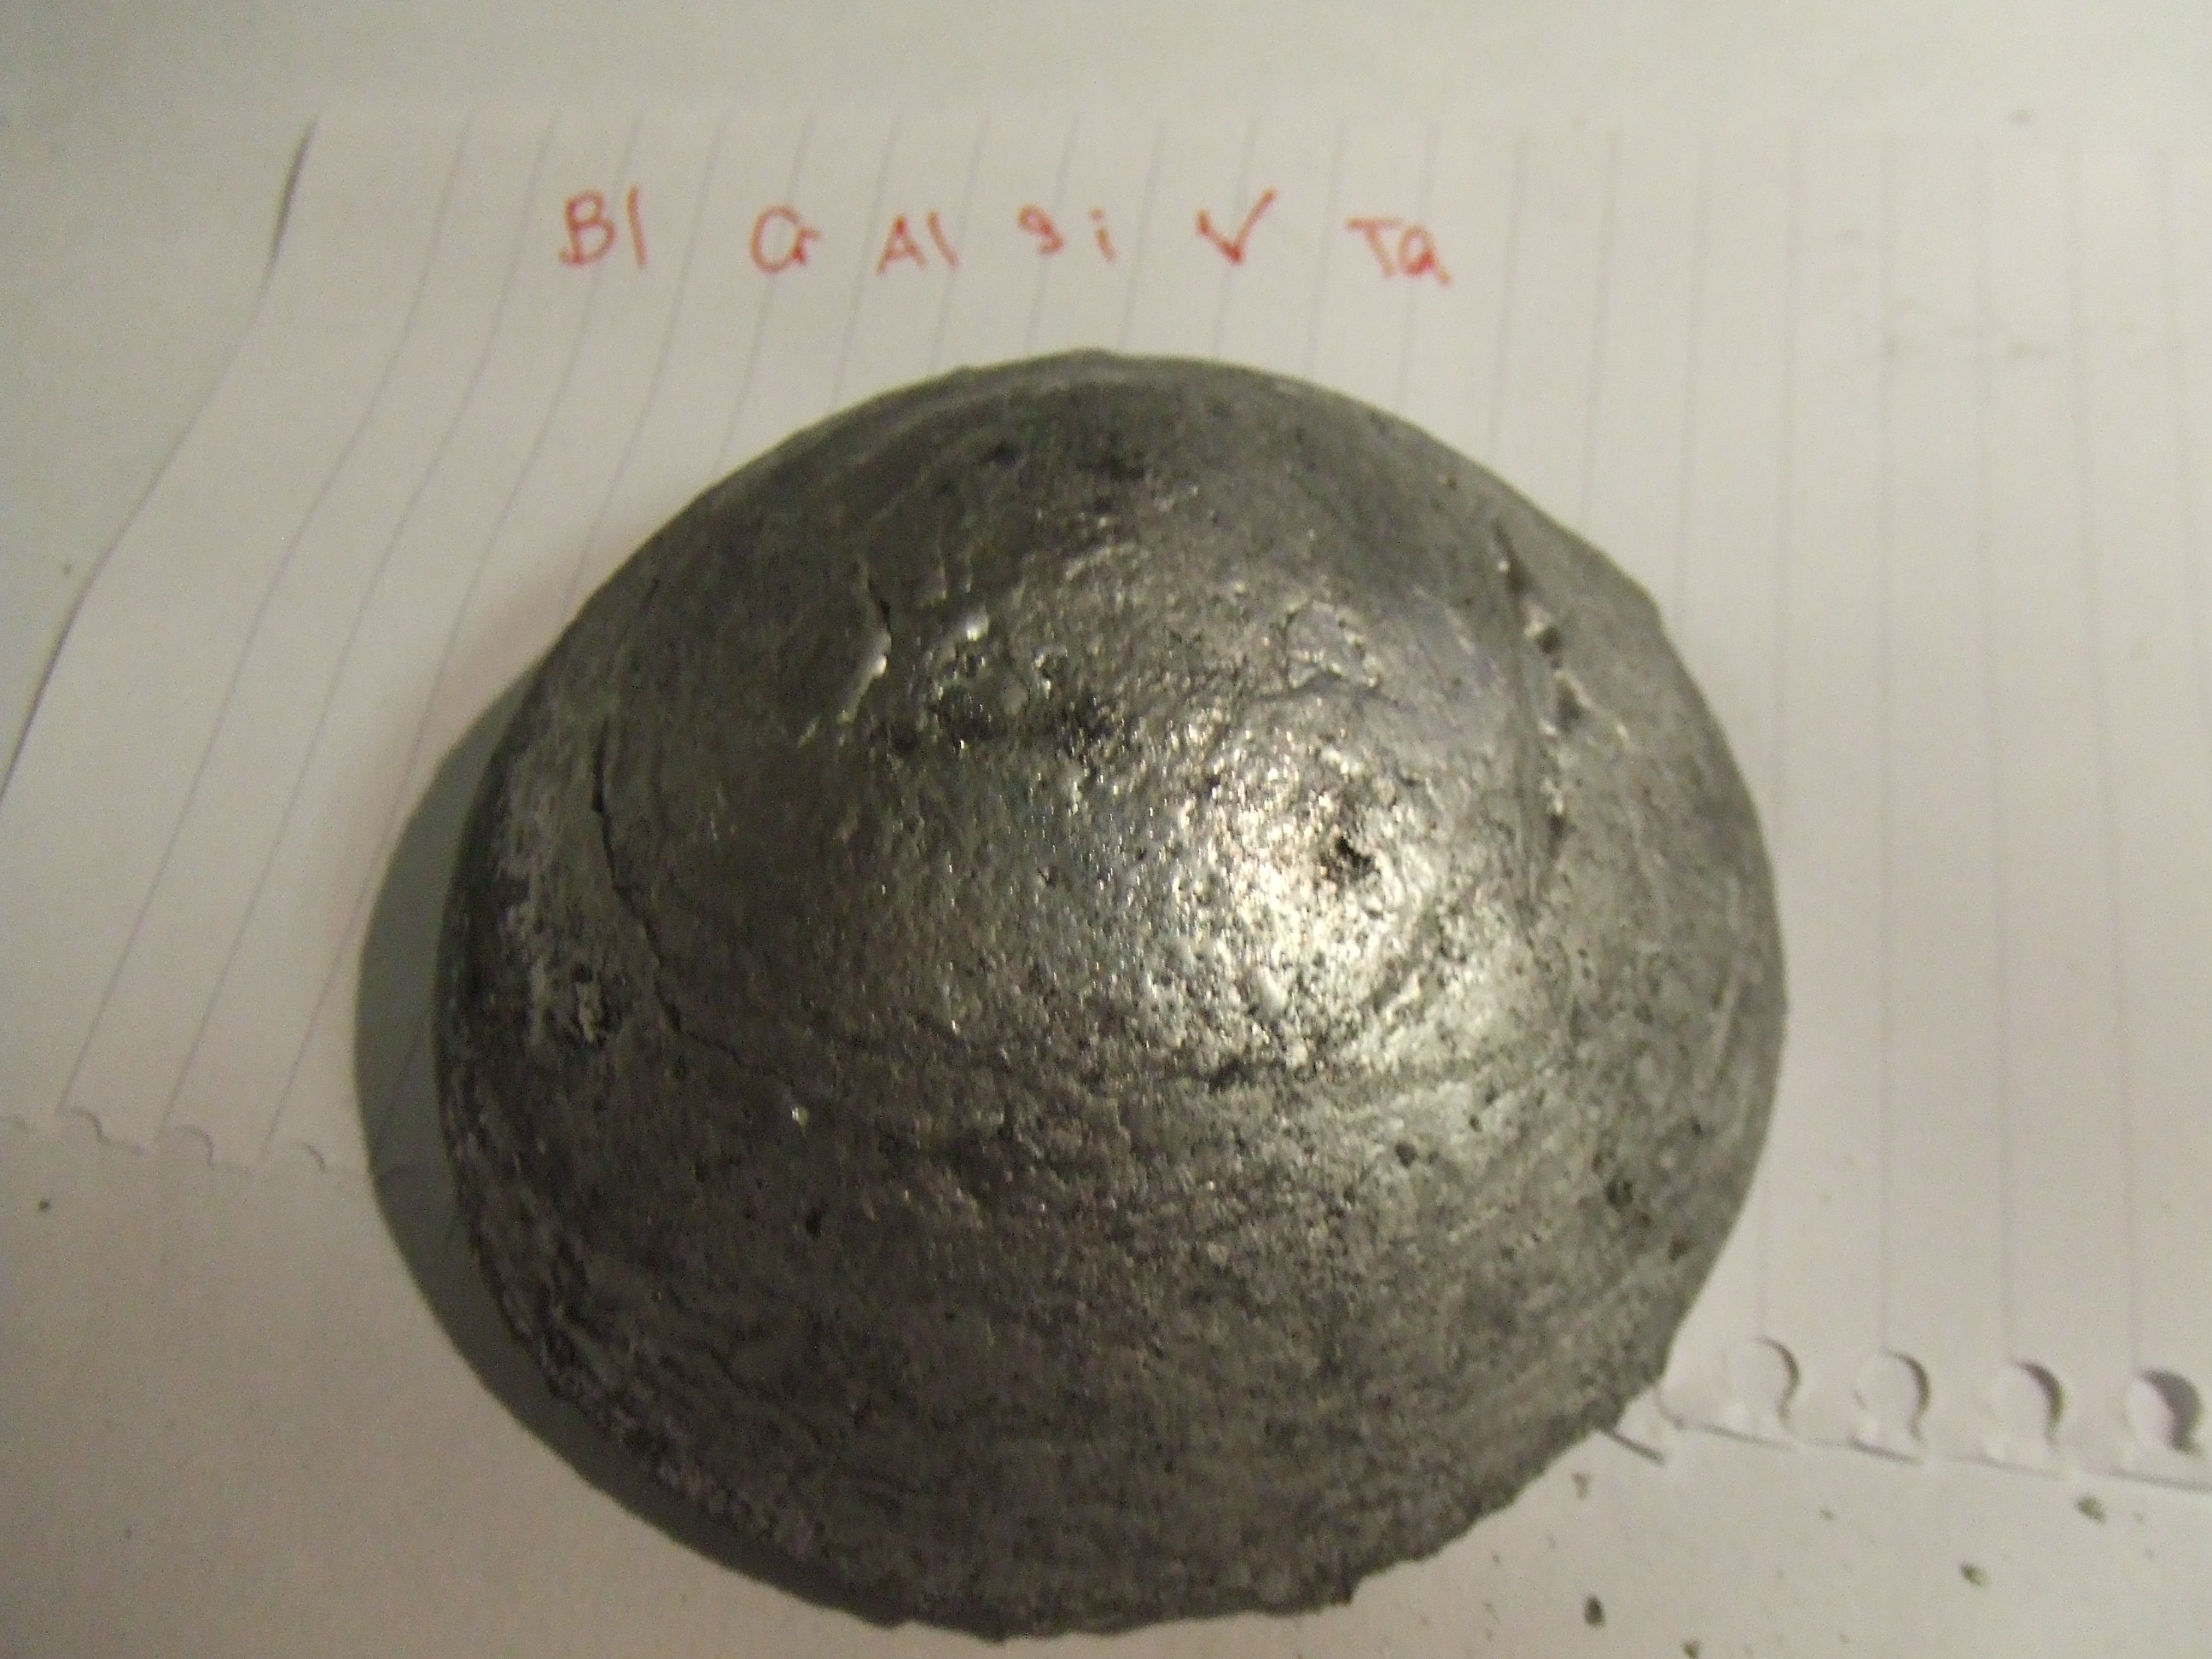
\includegraphics[width=7.8cm]{PMsanTaAl}
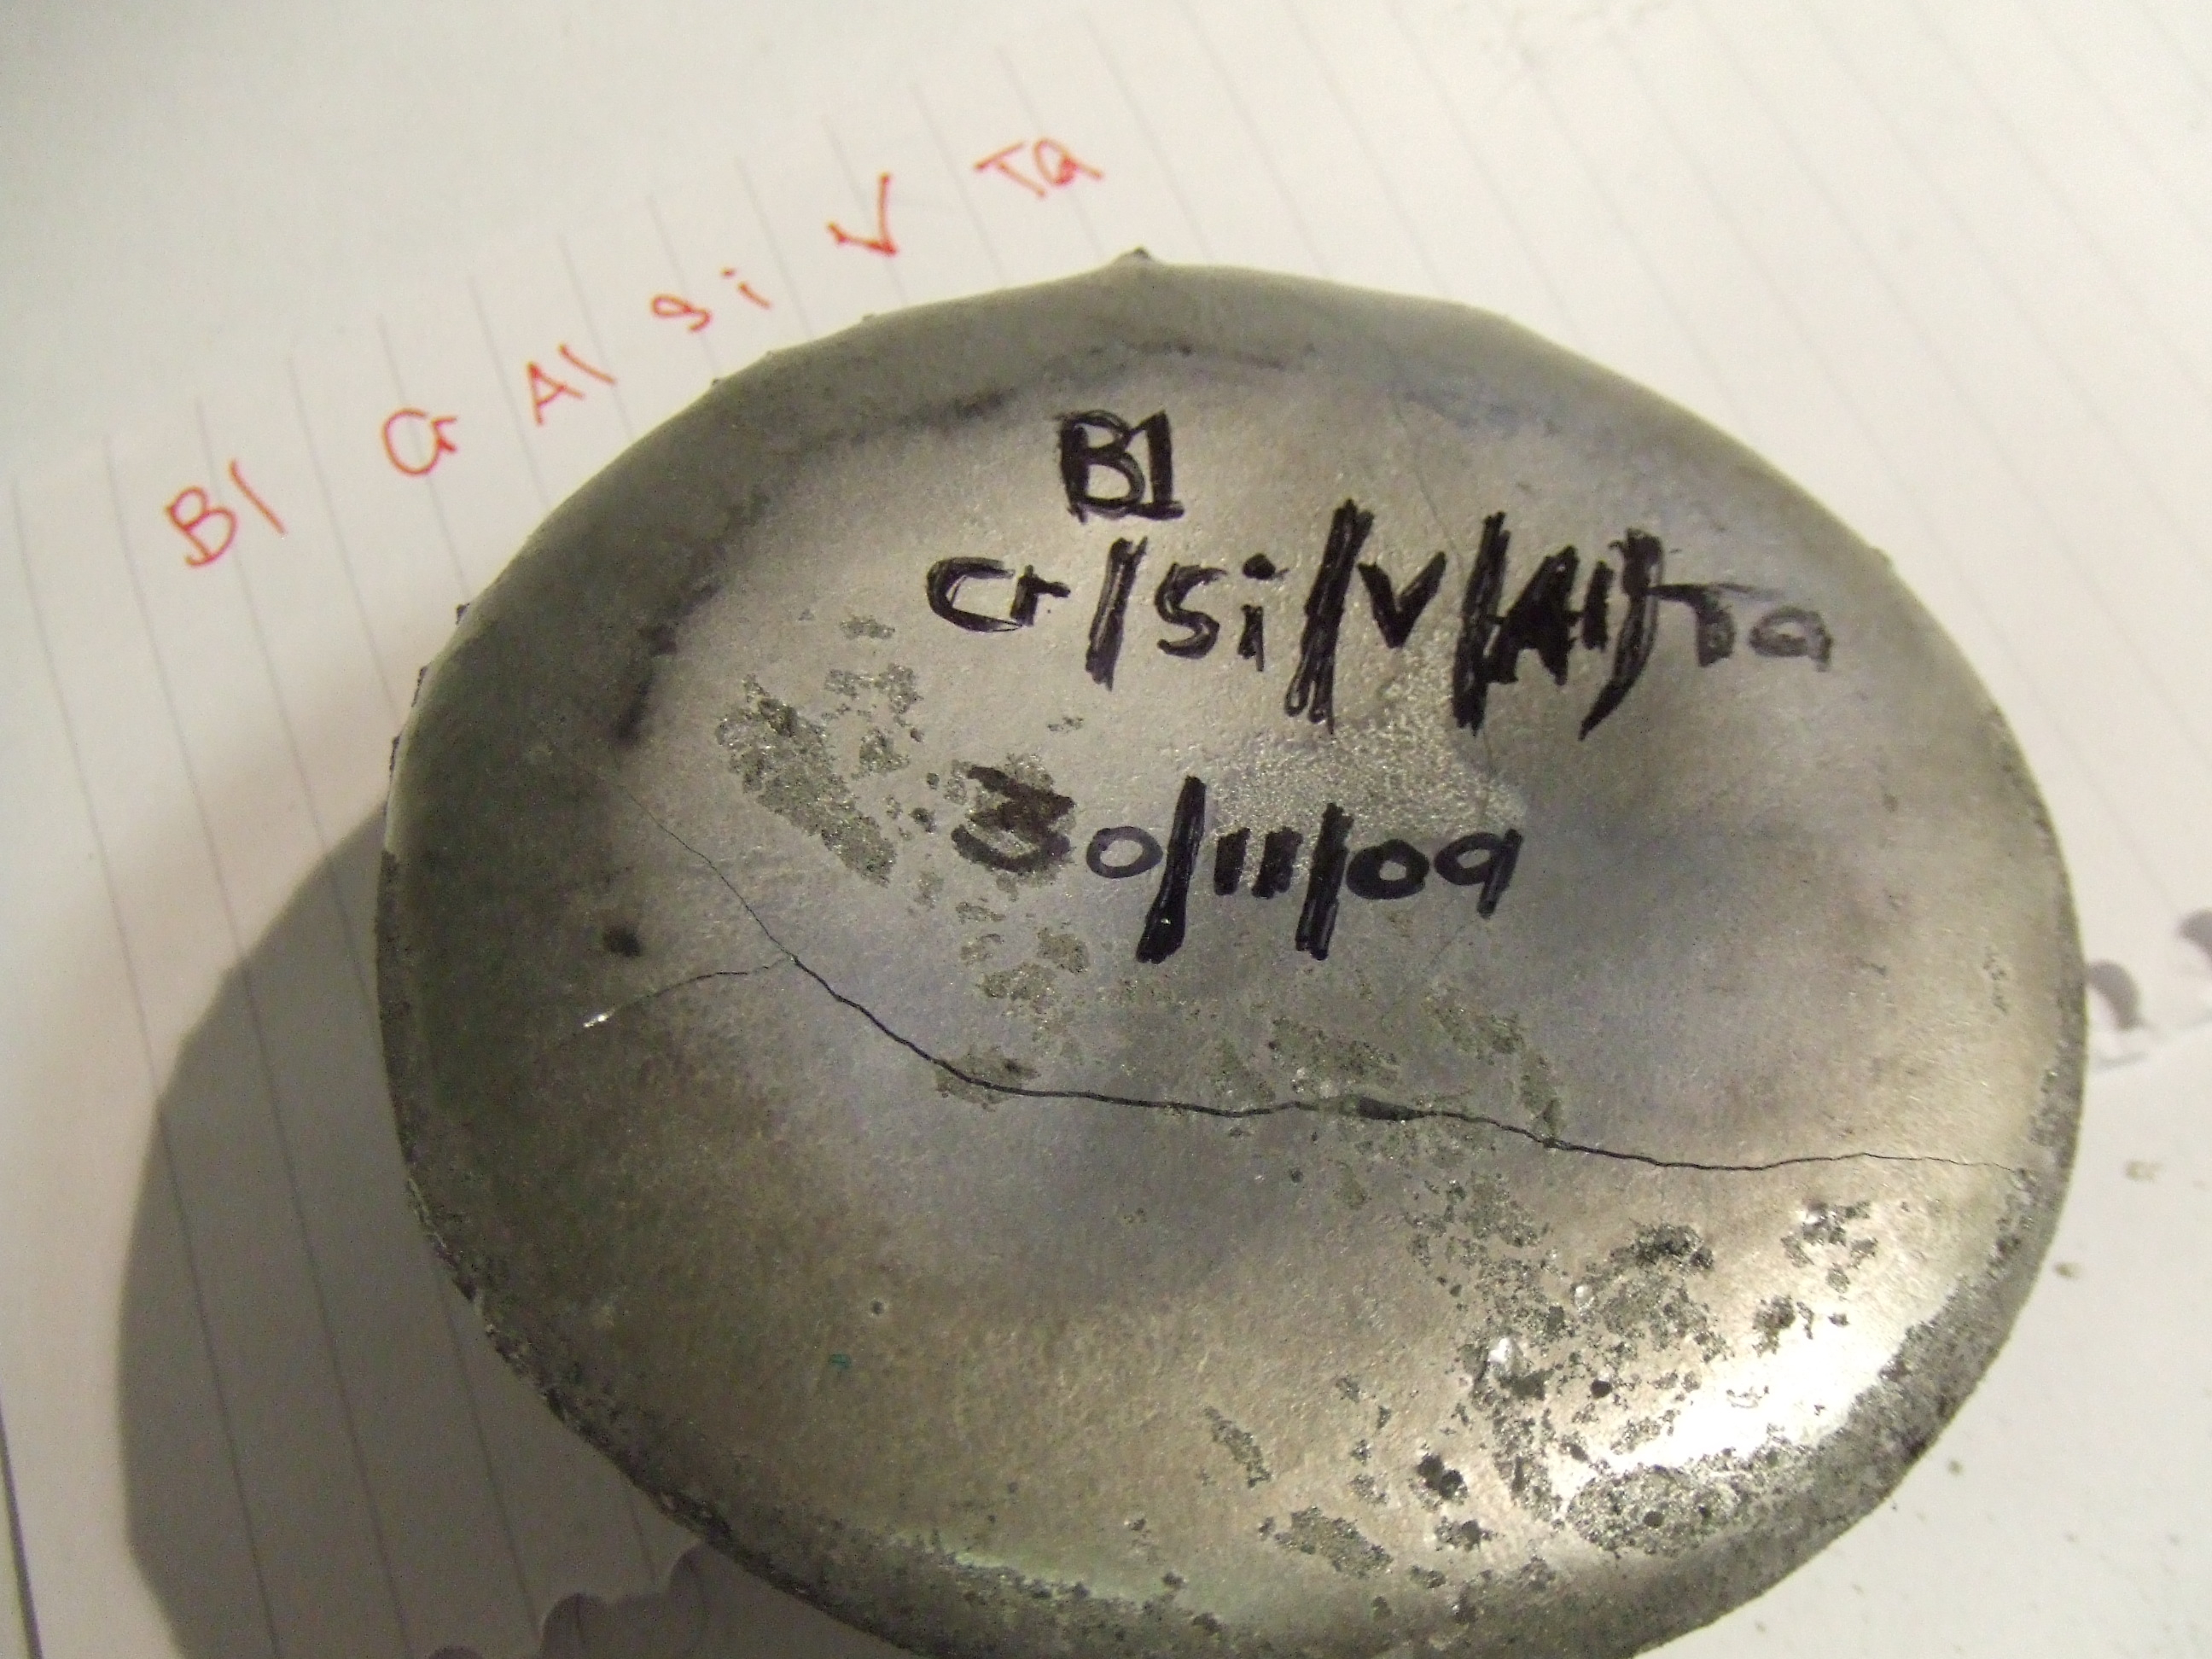
\includegraphics[width=7.8cm]{PMsanTaAlii}
\caption{Photographs of a \ilovewill{山}TaAl PM processed ingot displaying cooling cracks.}
\label{fig:pmsantaal}
\end{center}
\end{figure}
%
%
\begin{figure}[H]
\begin{center}
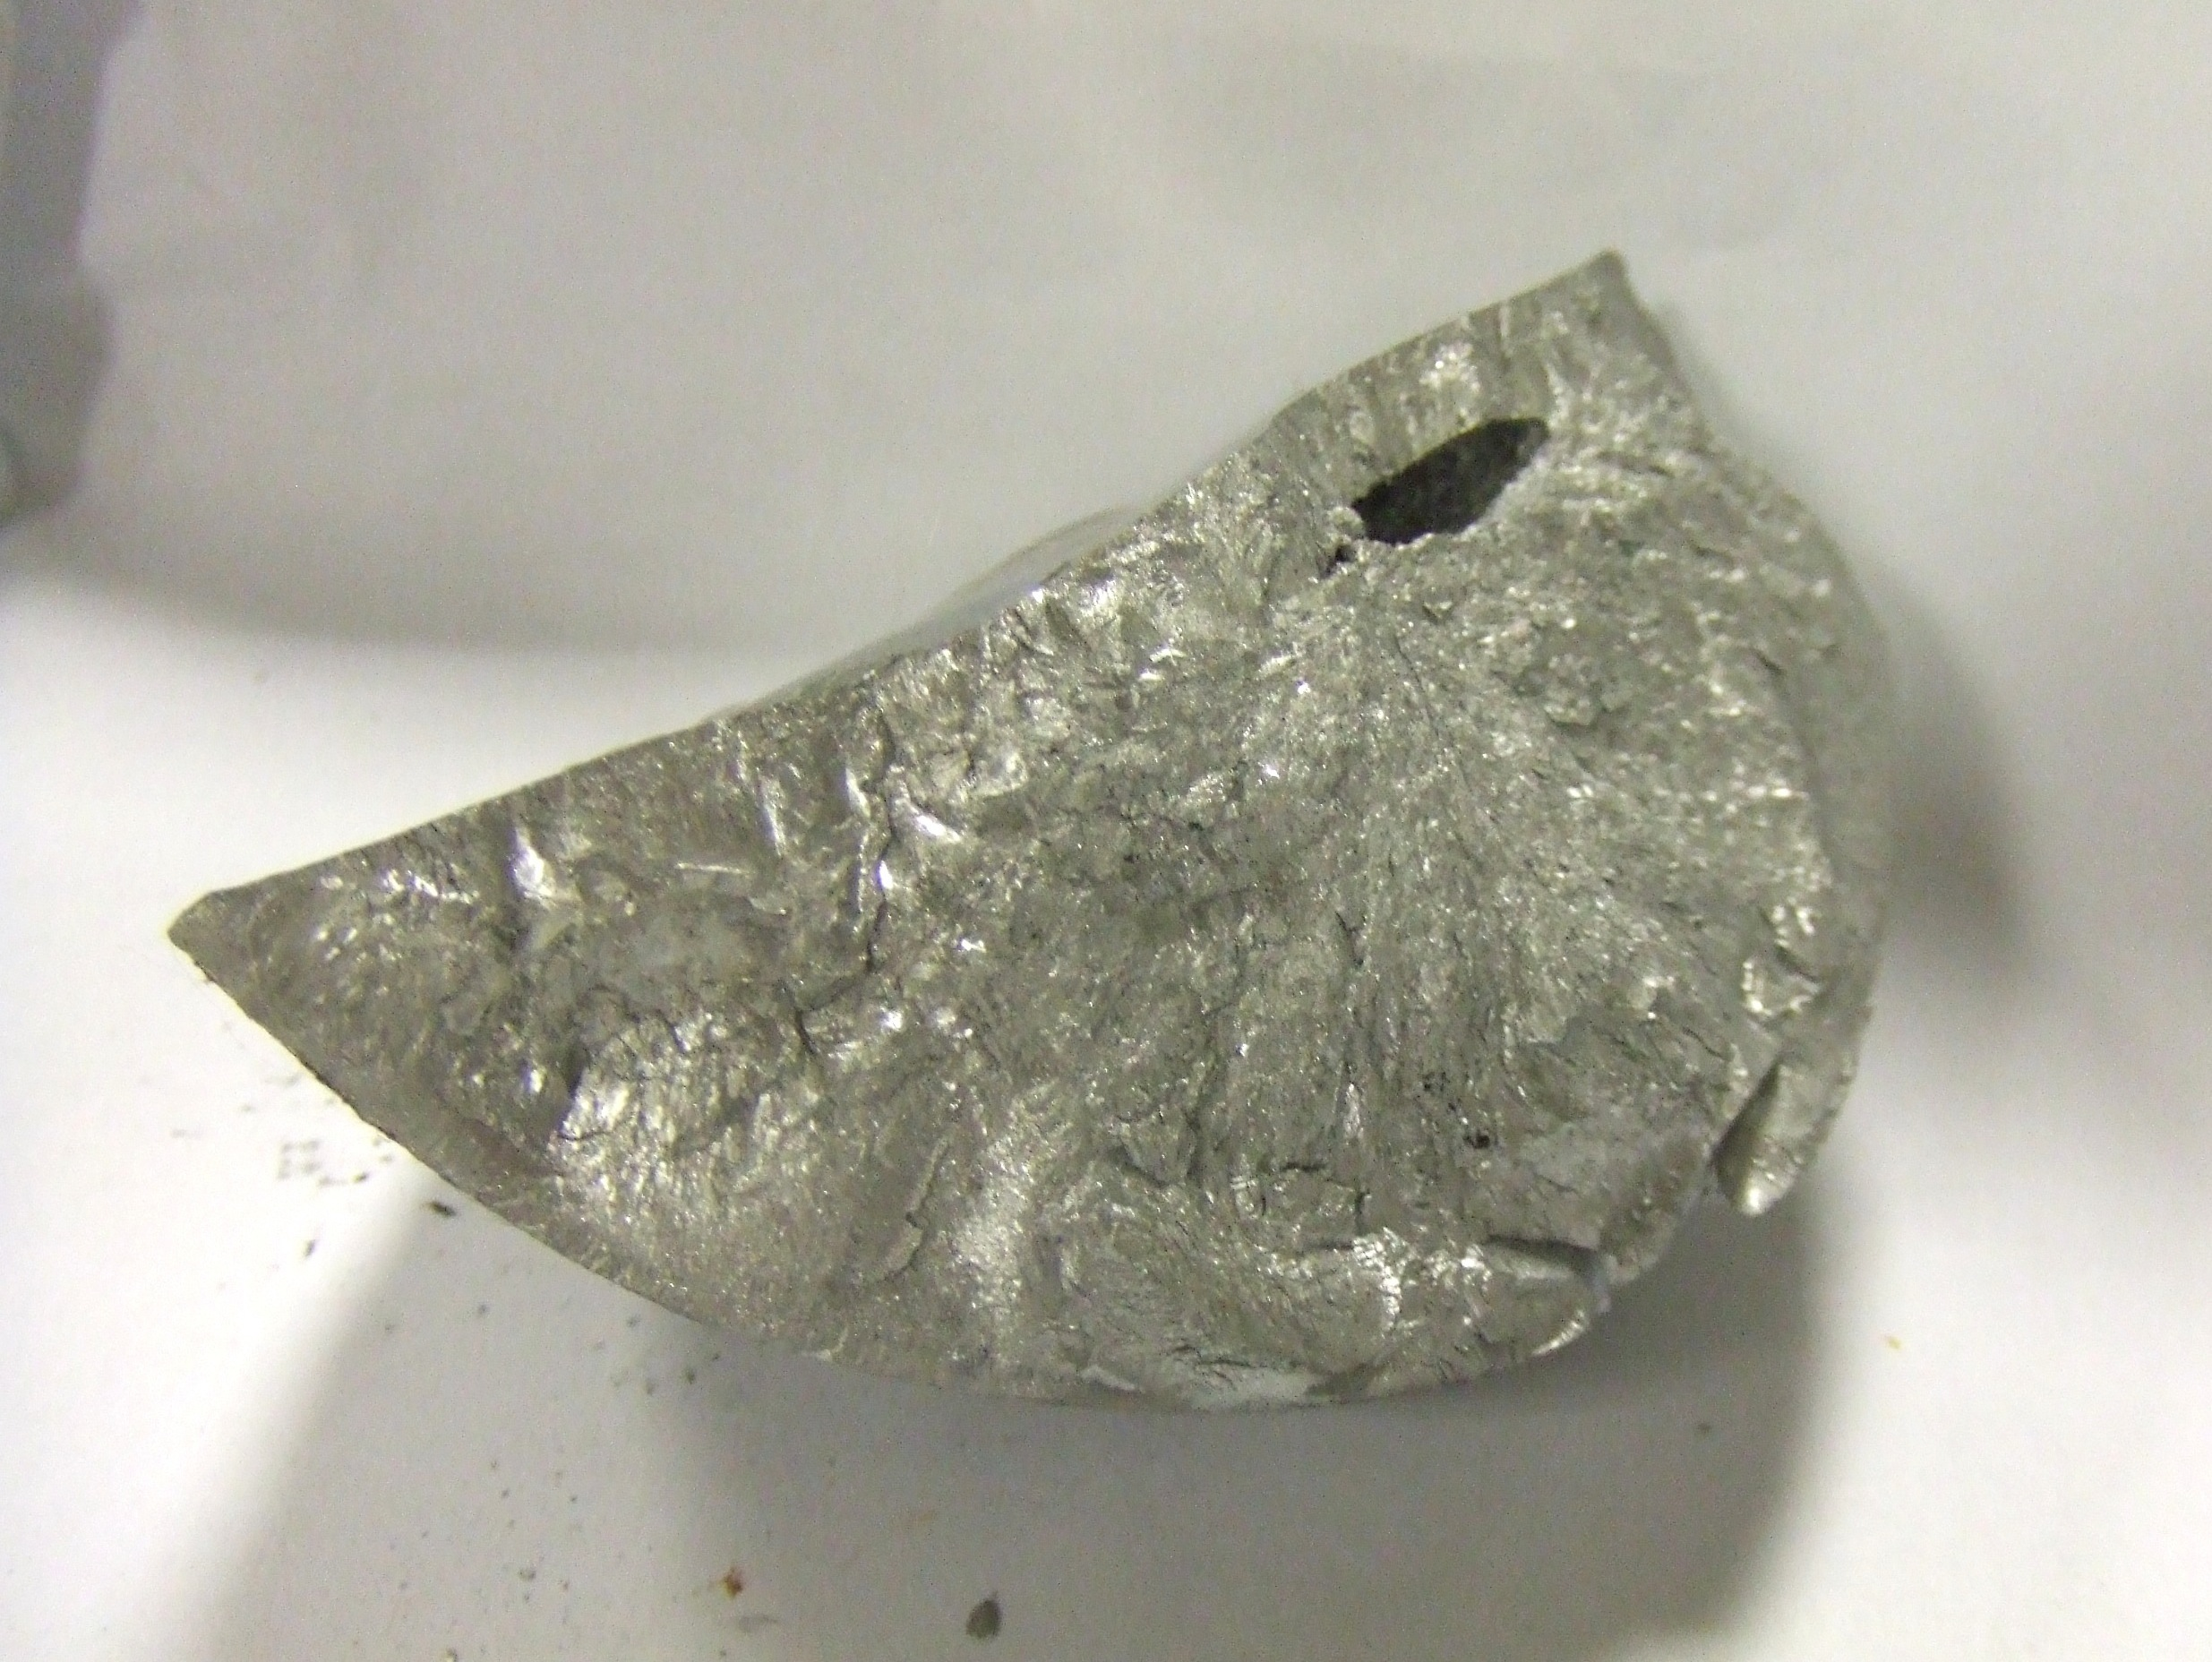
\includegraphics[width=7.8cm]{PMsanTaii}
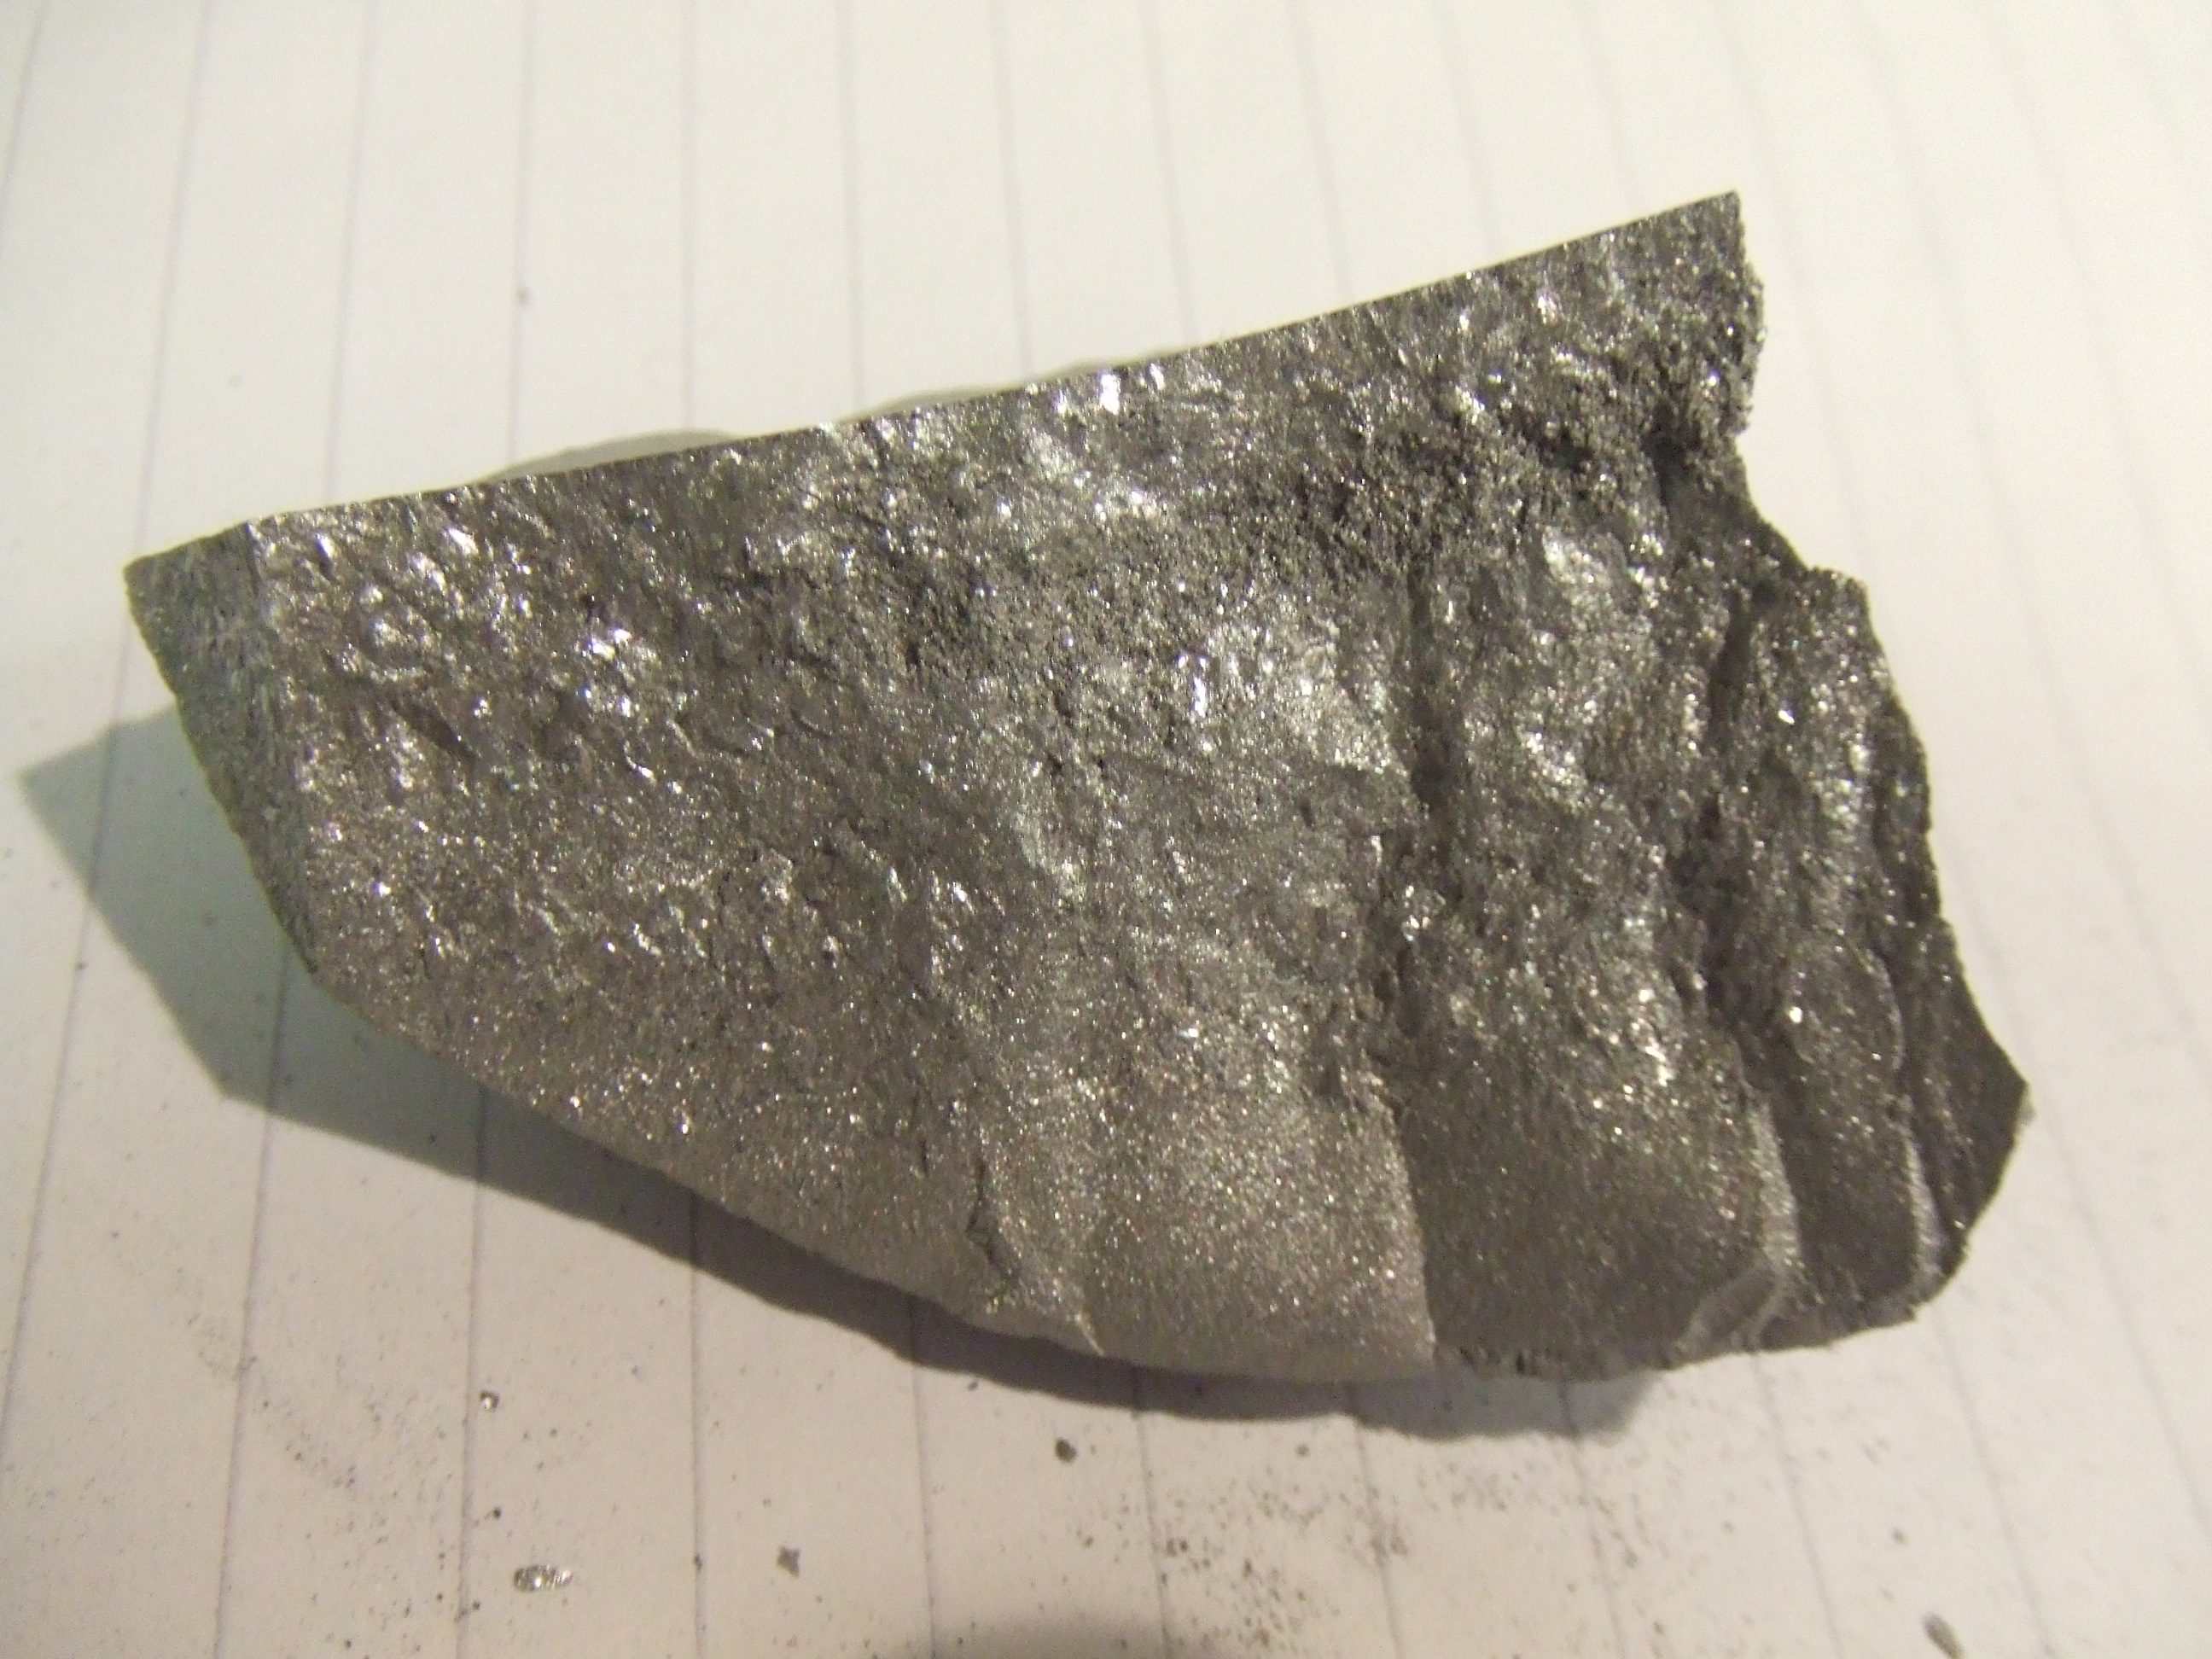
\includegraphics[width=7.8cm]{PMsanWAlii}
\caption{Photographs of PM processed ingots of (a) \ilovewill{山}Ta and (b) \ilovewill{山}WAl displaying inhomogeneity.}
\label{fig:pmsantaii}
\end{center}
\end{figure}
%
%
\begin{figure}[H]
\begin{center}
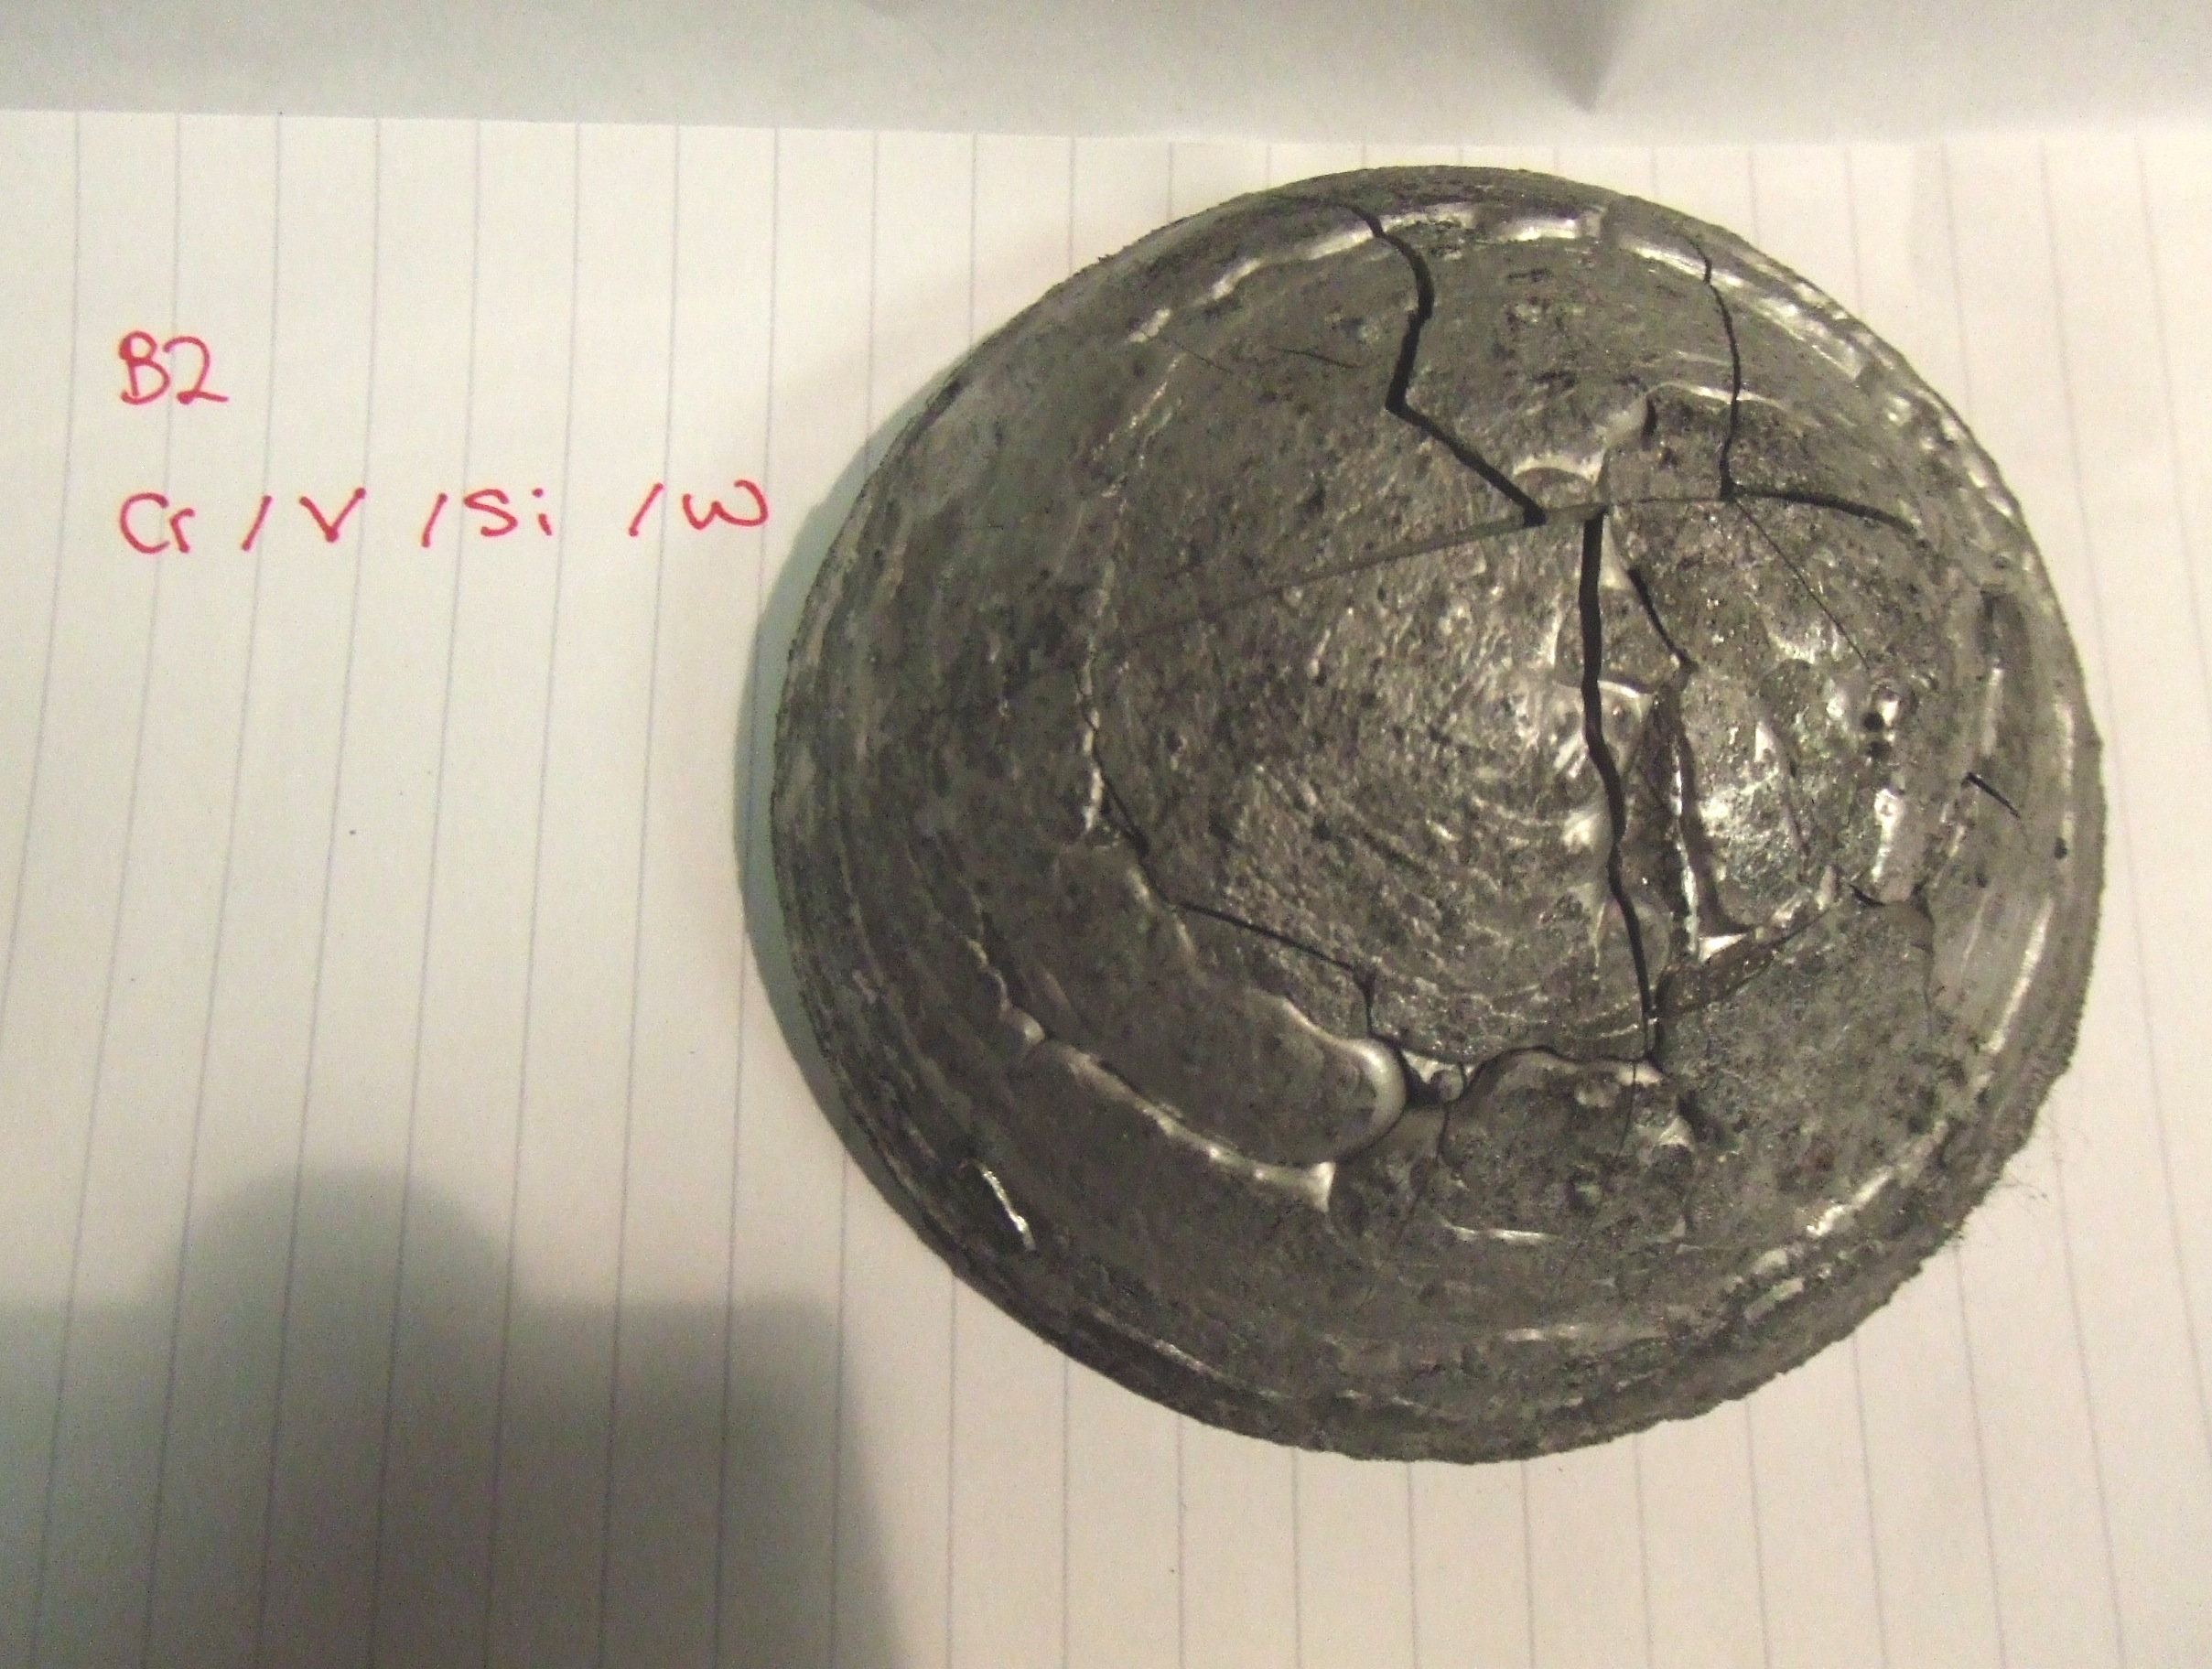
\includegraphics[width=7.8cm]{PMsanW}
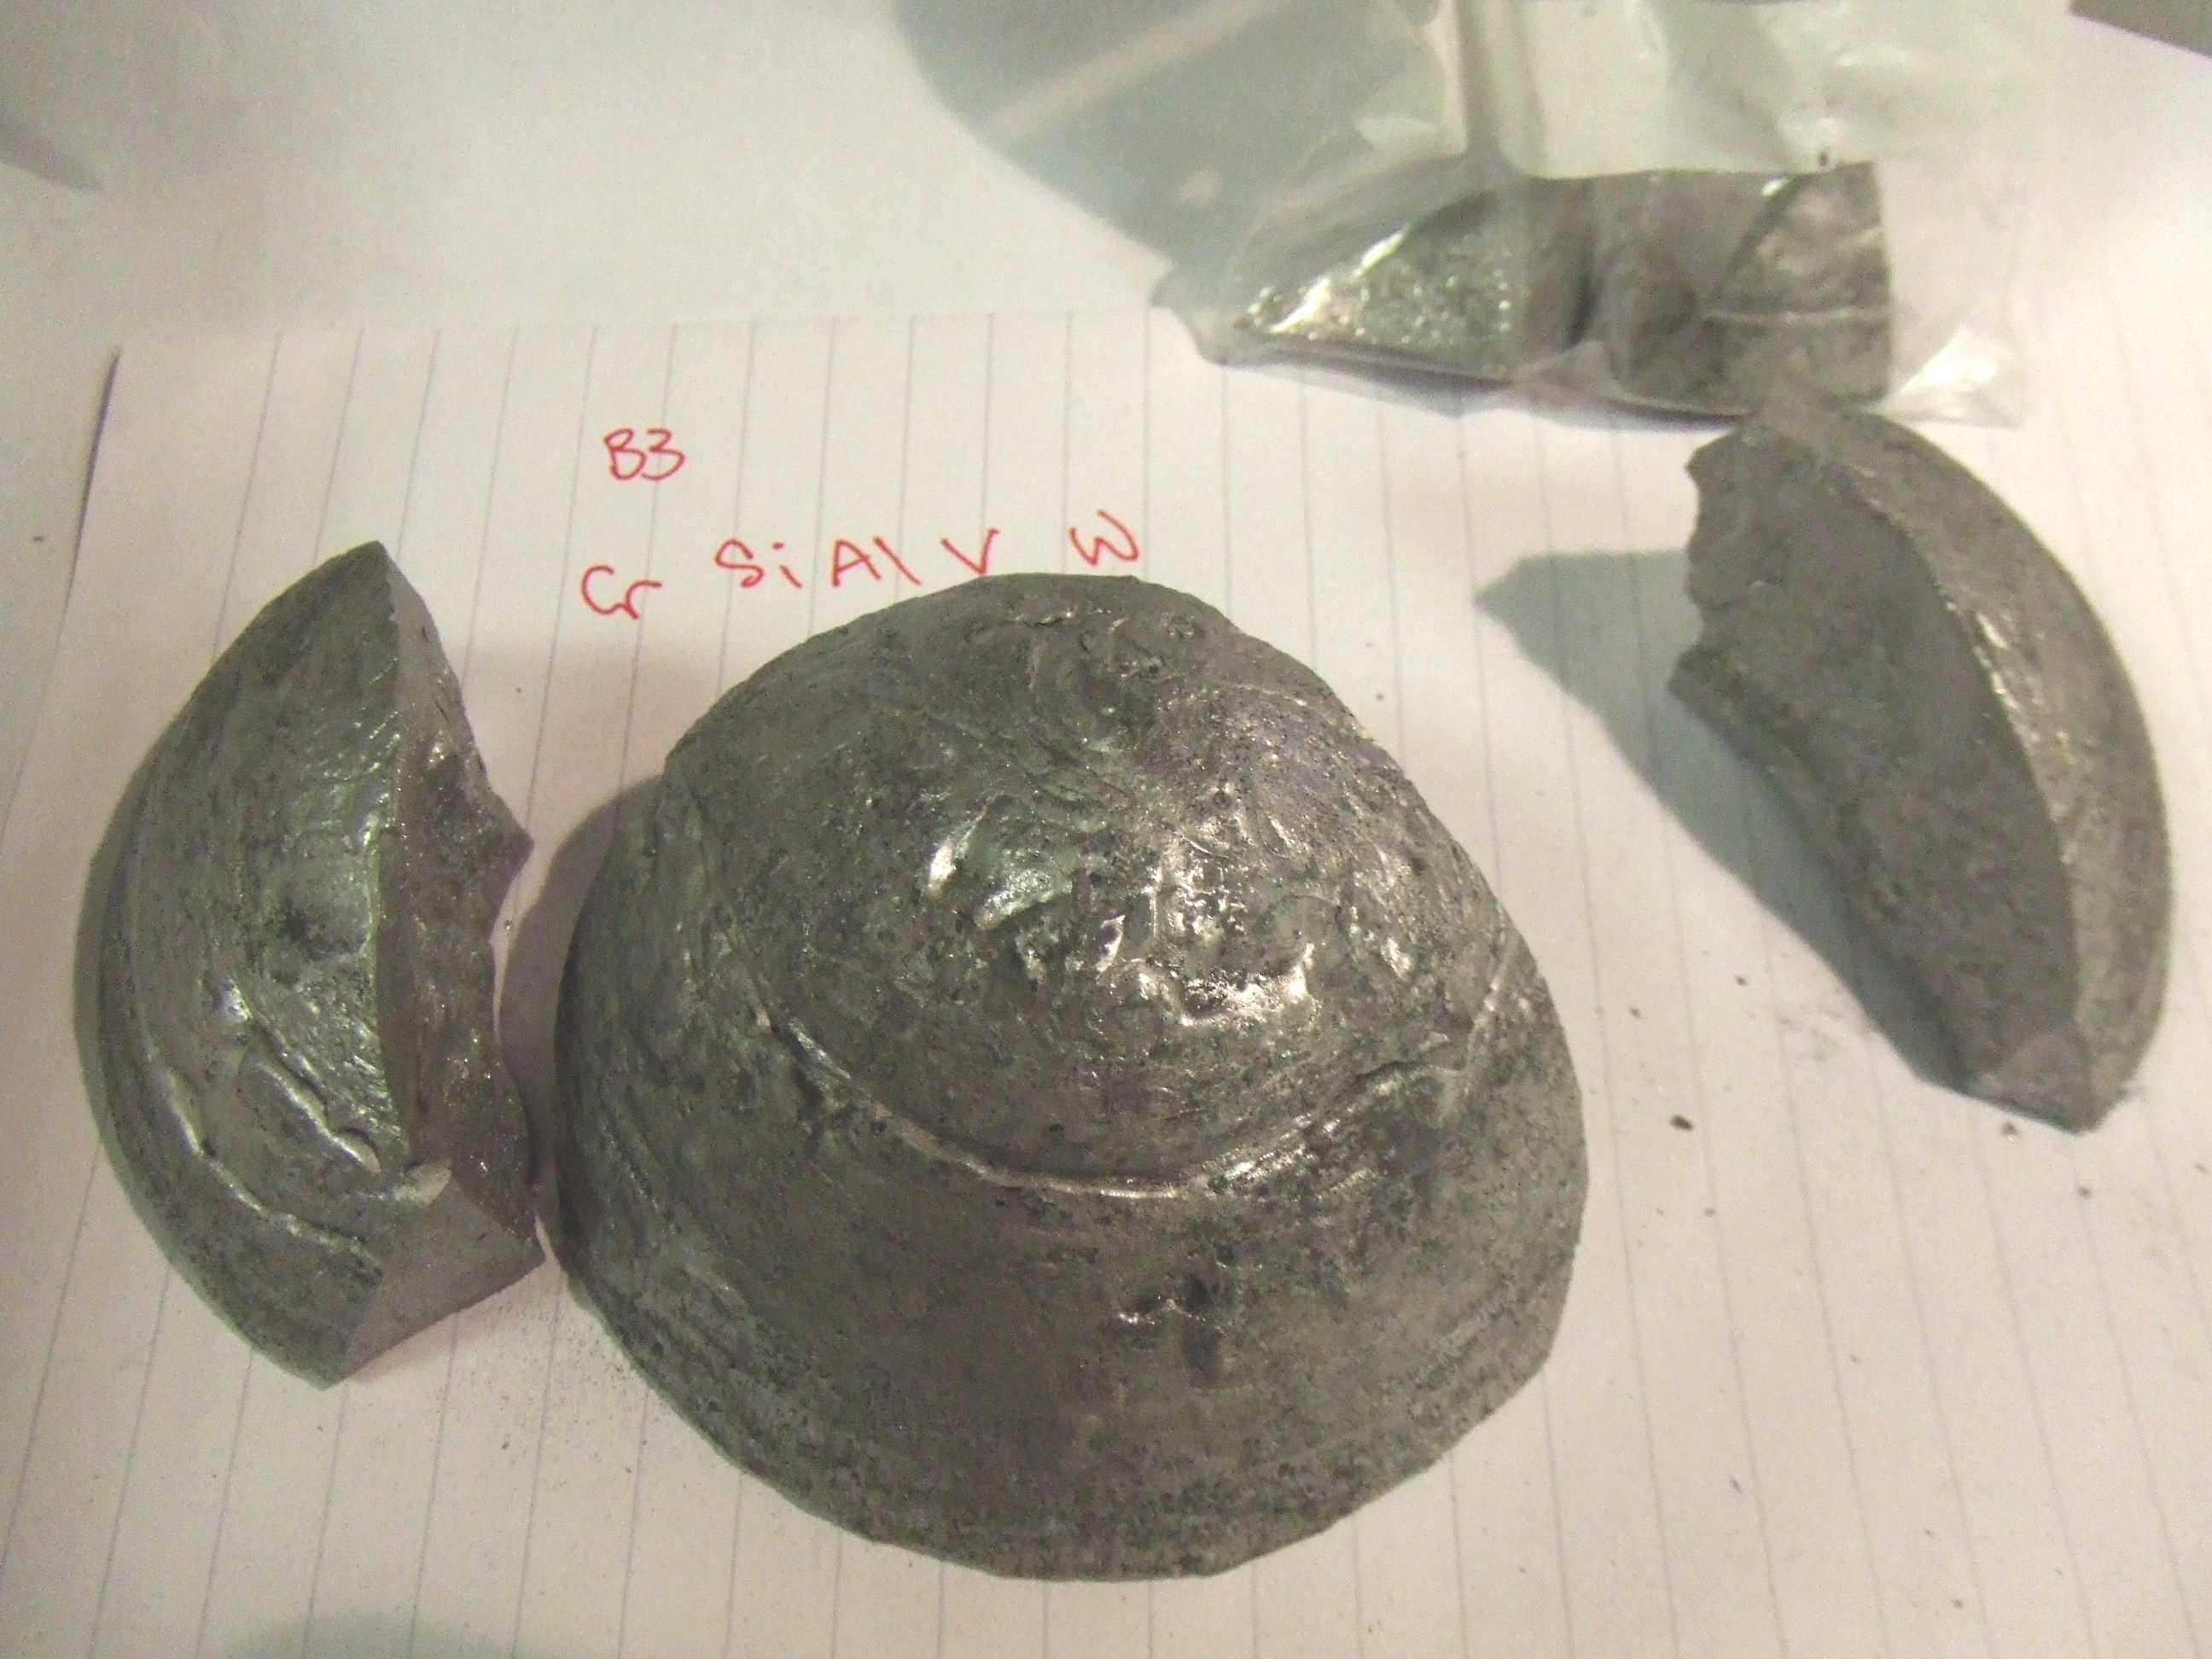
\includegraphics[width=7.8cm]{PMsanWAl}
\caption{Photographs of (a) \ilovewill{山}W and (b) \ilovewill{山}WAl PM processed ingots displaying through-specimen cooling cracks.}
\label{fig:pmsanw}
\end{center}
\end{figure}
%
\begin{table}[htdp]
\begin{center}
\begin{tabular}{llc}
\hline
Alloy 			&  Ingot Description		\\
\hline
Cr--Cr$_3$Si &cracked into several pieces, crumbly bits break off easily\\
V--V$_3$Si &minor crack in ingot, tough and not crumbly\\
\ilovewill{山}TaAl &minor cracks in ingot, tougher than Cr--Cr$_3$Si , not crumbly\\
\ilovewill{山}Ta &cracked into 7 pieces and crumbly bits chip off easily\\
\ilovewill{山}W &low surface tension, no meniscus, many cracks in ingot, not crumbly\\
\ilovewill{山}WAl &low surface tension, cracked into 4 pieces, not crumbly\\
\hline
\end{tabular}
\end{center}
\caption{Condition of as-cast ingots manufactured by the PM process.}
\end{table}




\subsection{Non-Directional Solidification Manufacture with the Vertical RF Furnace}

Arc-melt ingots were used as feedstock initially.  They were found to be inhomogeneous.  PM manufacture stock was used as feedstock in the newer specimens. 
 
Two castings of the Cr--Cr$_3$Si eutectic were done using the radio frequency furnace in Cambridge.  The first cast was allowed to equilibriate at 1740\celsius, 35\celsius\ above eutectic melting point, for 1 hour, before being withdrawn at 20 mm/h.  When the alumina crucible was broken open after the cast, the feed arc-melt ingot was found to have only partially melted.  The hold time was possibly not long enough for the ingot to melt, and the hot zone could be smaller than the feed ingot, and only the portion within the hot zone melted.  The second cast was equilibriated at 1780\celsius\ for an hour.  A better melt was achieved before this cast.  Peering down the opening of the cylindrical crucible, a meniscus was seen.  Under the circumstances, that was the best measure of the degree of melting of the feed ingot.  This ingot was also solidified at 20 mm/hr.  Due to reaction between the alumina crucible and cast ingot, the ingot had to be broken out of the crucible.  This ingot seemed to have been cast well.  Microstructural and compositional analysis have not been performed on the ingots yet, due to difficulties in getting the ingot cut.  The electro-spark machining equipment at the department were unsuccessfully employed.  The samples had to be out-sourced for machining.
%
\begin{figure}[H]
\begin{center}
\includegraphics[width=8cm]{rfsmall}
\caption{Photographs of a Cr--Cr$_3$Si arc-melt ingot that was non-directionally solidified in the in-house vertical RF furnace and experienced incomplete melting.}
\label{fig:rfsmall}
\end{center}
\end{figure}
%

\section{Directional Solidification Manufacture}

It was hypothesised that a lamellar microstructure aligned to the loading axis would be able to partition load to the silicide phase effectively.  In order to accomplish this, pull-rates have to be very low to maintain the suitable growth front required.  This invariably leads to microstructure coarsening.  The various attempts at DS met with limited success due limitations of temperature capability, the lack of a mixing mechanism for the melt, and the lack of homogeneous feed-stock.  


\subsection{Directional Solidification with the Vertical RF Furnace}

Zirconia-coated alumina crucibles were also tried, with a maximum casting temperature of 1760\celsius.  This is a temperature that alumina can withstand without adverse effects.  The crucible underwent a reaction with itself at 1760\celsius.  The crucible lip, which was not in contact with the feedstock, melted, splitting and curling downward.  A small piece of the alumina crucible holding this compromised crucible chipped off, and hit the water-chilled double-walled silica containment vessel.  This alumina piece was at a temperature close to 1760\celsius, and its impact with the inner silica wall induced sufficient thermal shock to initiate the catastrophic failure of the silica vessel.  A bespoke replacement of the silica vessel had to be made before the furnace could come back on-line.  This process took three months.

%
\begin{figure}[H]
\begin{center}
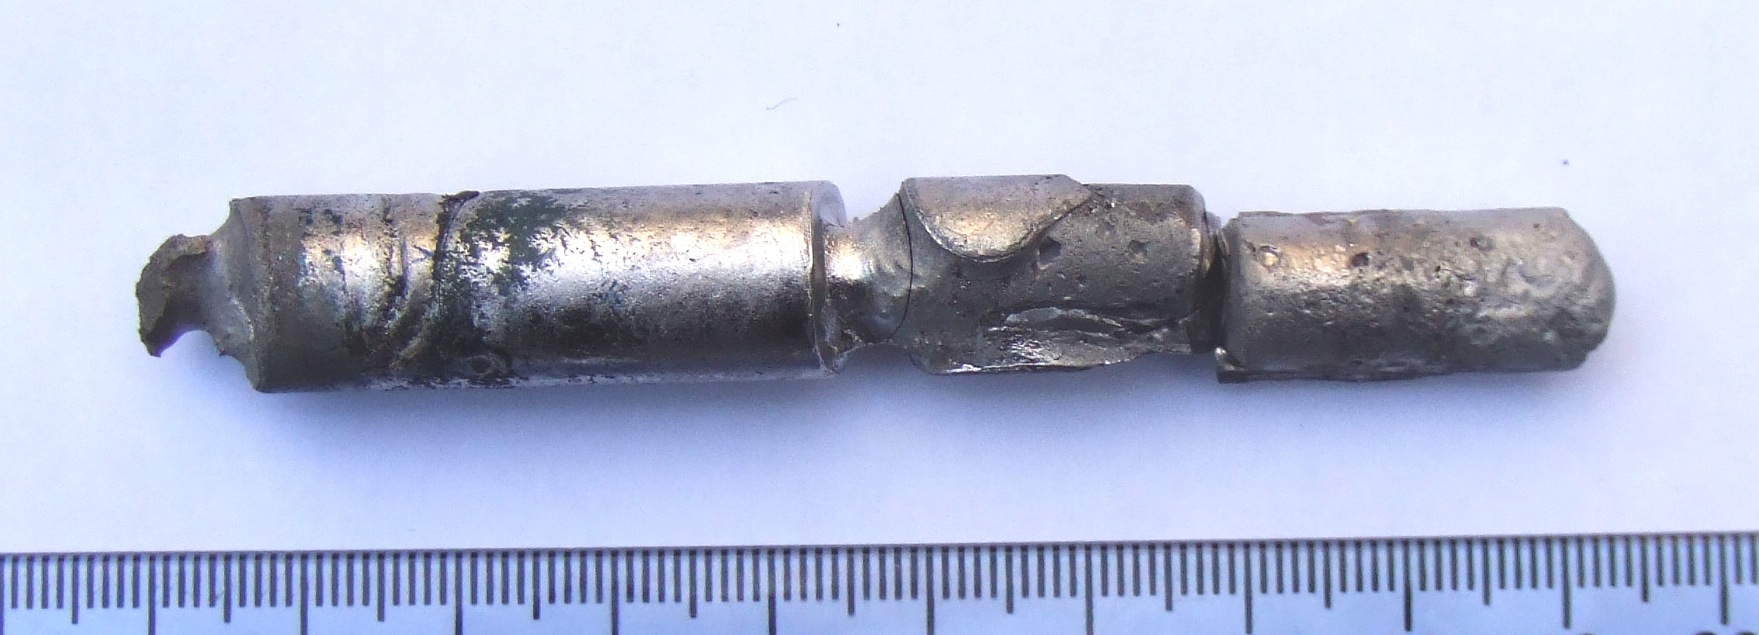
\includegraphics[width=10cm]{rfi}
\caption{A photograph of a typical directionally solidified cast cylindrical specimen manufactured using the in-house vertical rf furnace.}
\label{fig:rfia}
\end{center}
\end{figure}
%

The recommended maximum operating temperature of the in-house RF furnace is 1800\celsius.  In order to preserve the life-time of the furnace, it has never been run at temperatures above 1600\celsius.  We were hesitant to push it to the maximum recommended temperature as the temperature is controlled manually.  If sudden runaway temperature increases occur, there will not be an automatic cut in power to curtail the temperature ramp. Exceeding the maximum temperature would be probable if feedstock had to be melted at 1800\celsius, especially since furnace temperature fluctuations are greater at higher temperatures.  Although we readily discovered that 1760--1790\celsius\ was insufficient to completely melt feedstock, furnace fluctuations of 40\celsius\ proved difficult to control at 1800\celsius, and only two or three ingots were manufactured at this temperature.  The RF furnace has a definite hot zone, and an initial pass of the feedstock through this hot zone was incorporated into subsequent alloy manufacture attempts, as much as the furnace constraints would allow.  

DS \ilovewill{山}W (Figure \ref{fig:sanw})  manufactured using the in-house RF furnace has a very high melting point.  The 1780\celsius\ capability of the RF furnace was not high enough to induce sufficiently low melt viscosity to allow the composition to solidify as a rod.
%
\begin{figure}[H]
\begin{center}
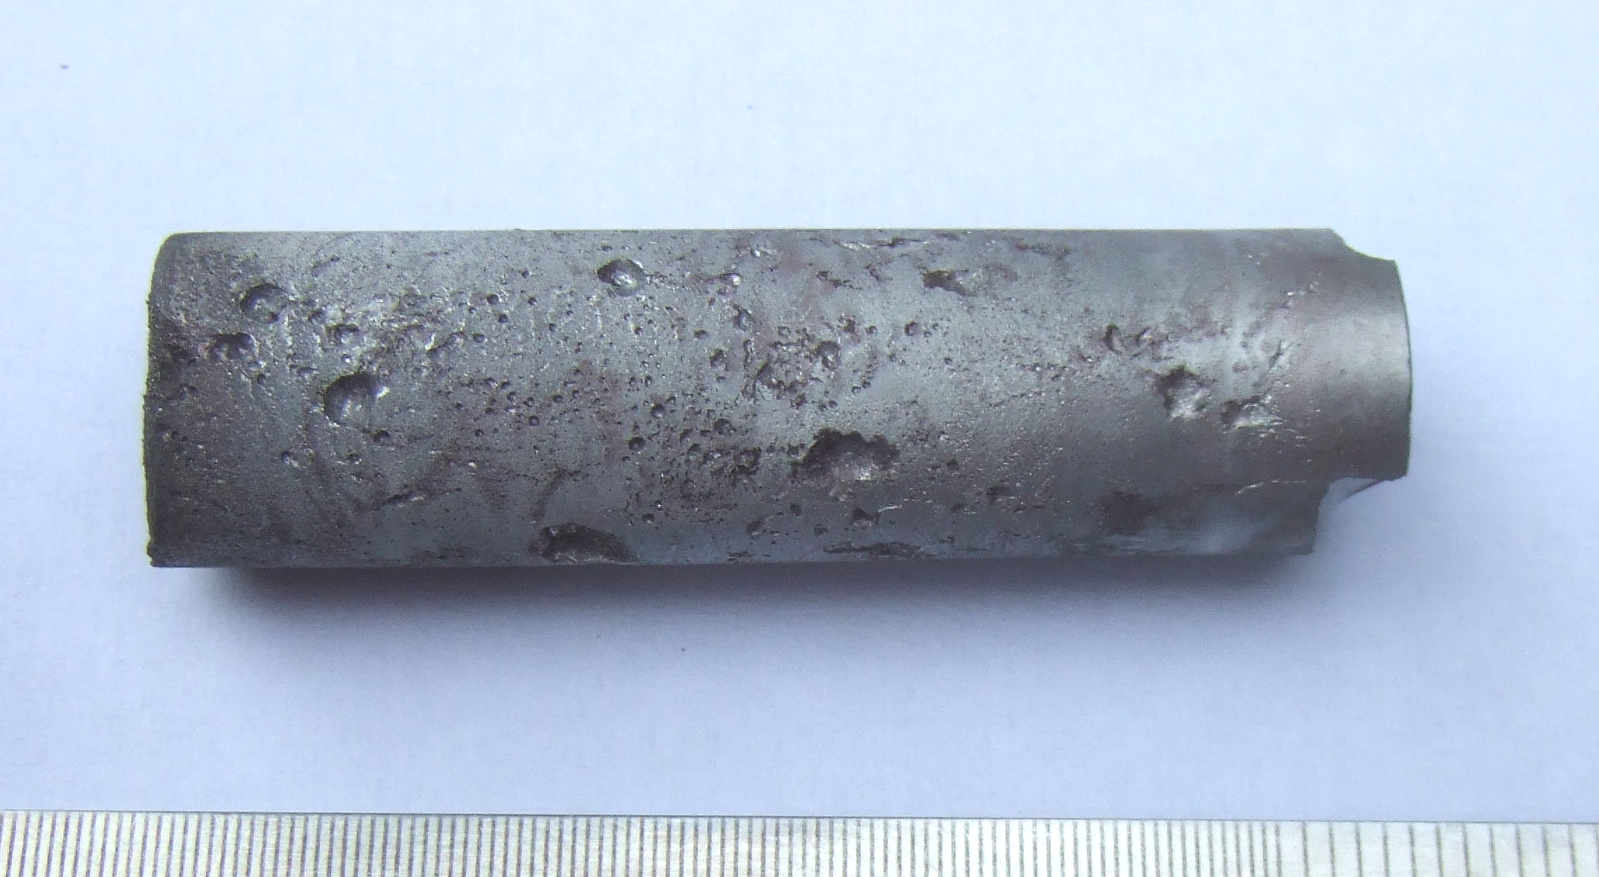
\includegraphics[width=9cm]{santarf}
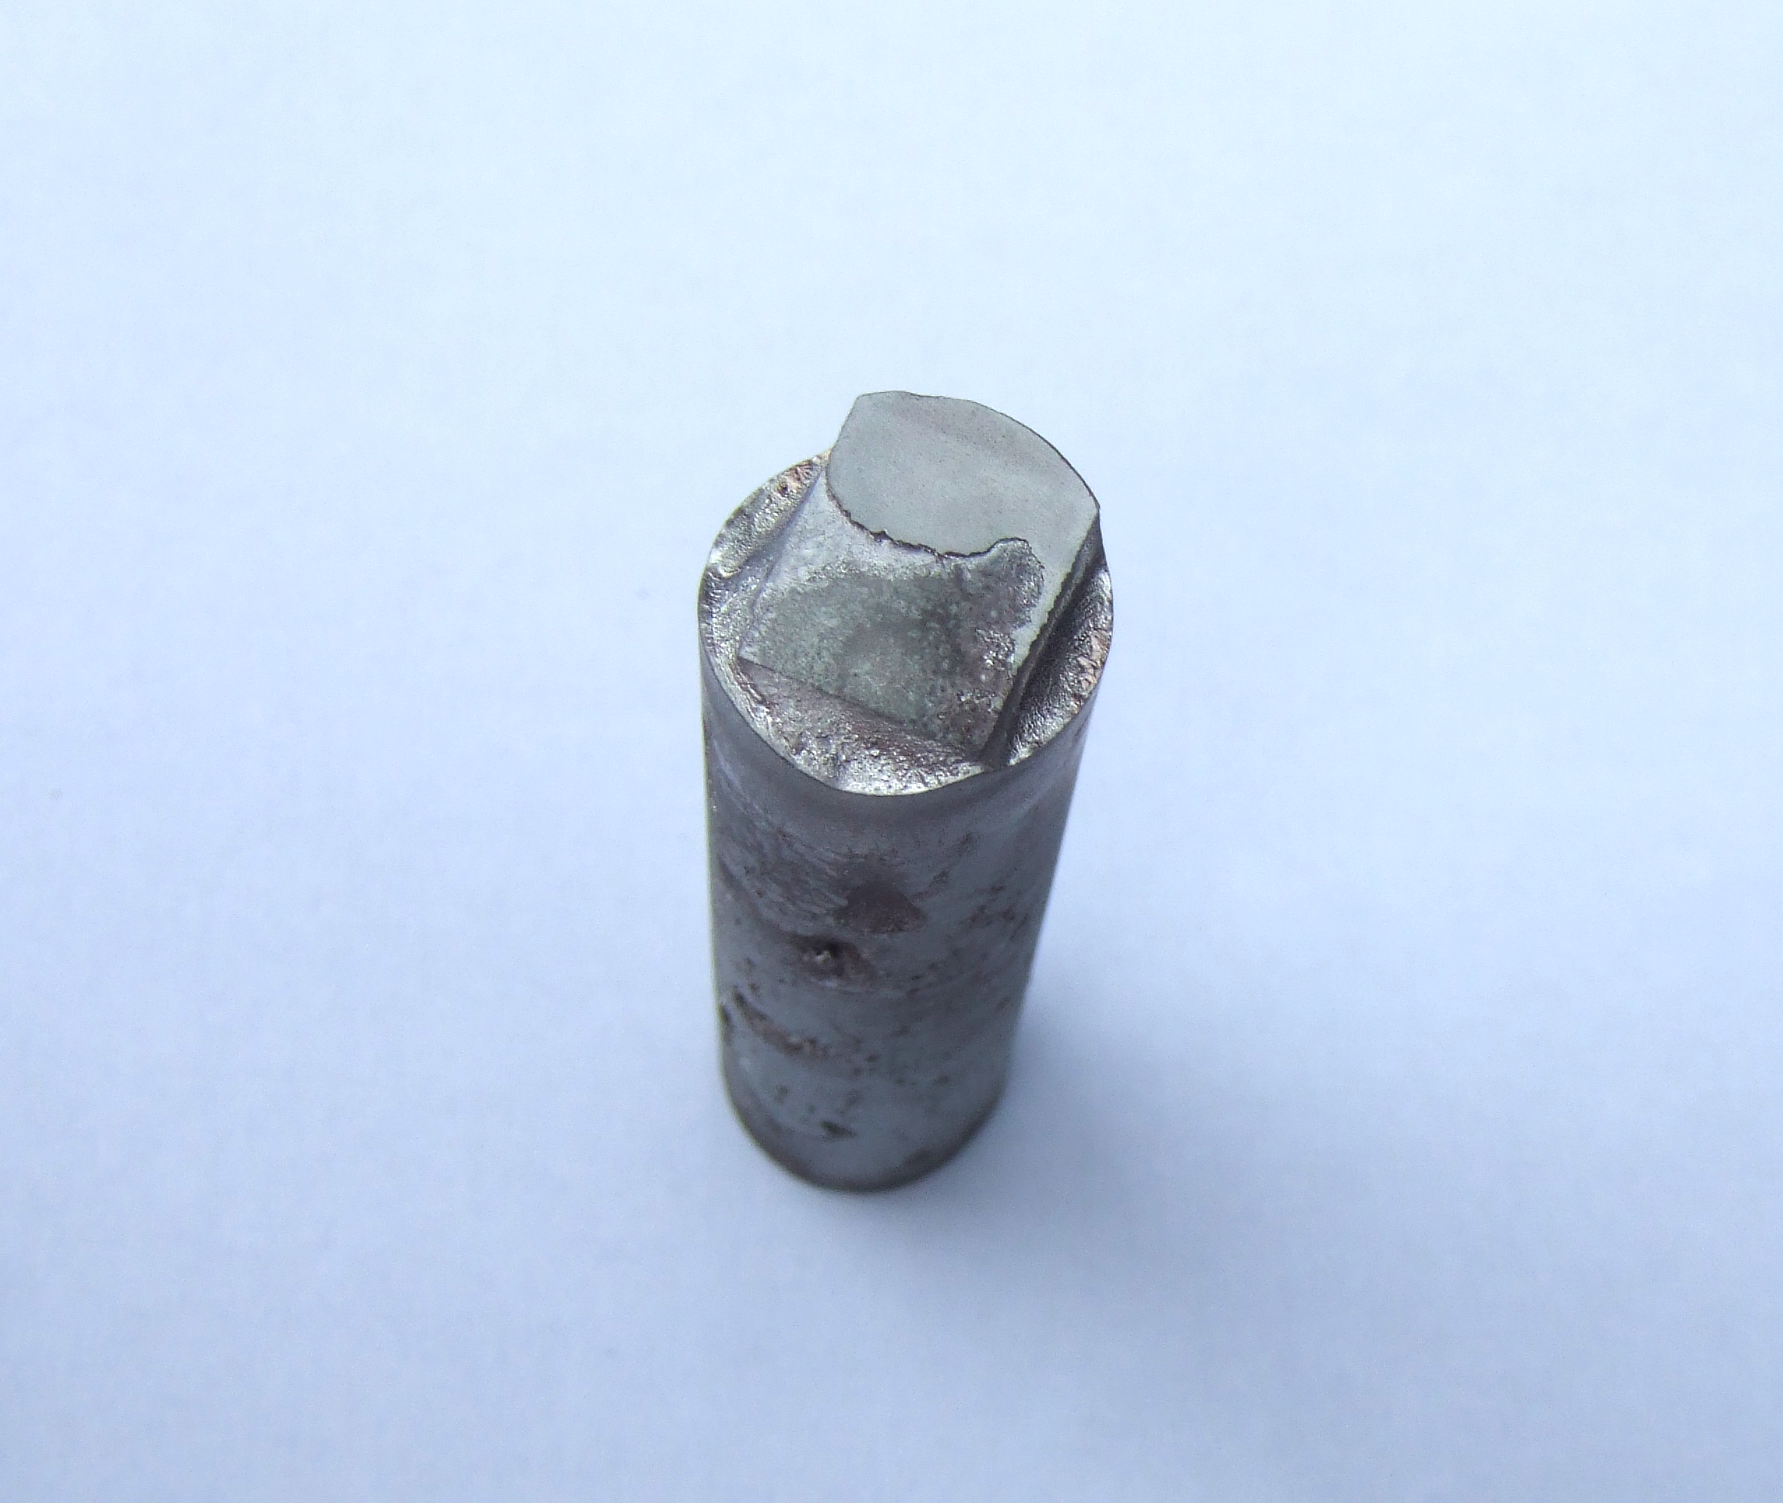
\includegraphics[width=6cm]{santarftop}
\caption{(a) the long view of an ingot of \ilovewill{山}Ta by DS manufacture using the in-house RF furnace, made with PM manufactured feed-stock. This was melted at about 1785\celsius\, drawn at 30milli\metre\/h to melt and somewhat homogenise the feedstock, and re-drawn at 30\milli\metre\/h.  (b) the top view of the ingot, showing unmelted feedstock due to limited furnace temperature capability.}
\label{fig:santarf}
\end{center}
\end{figure}
%
%
\begin{figure}[H]
\begin{center}
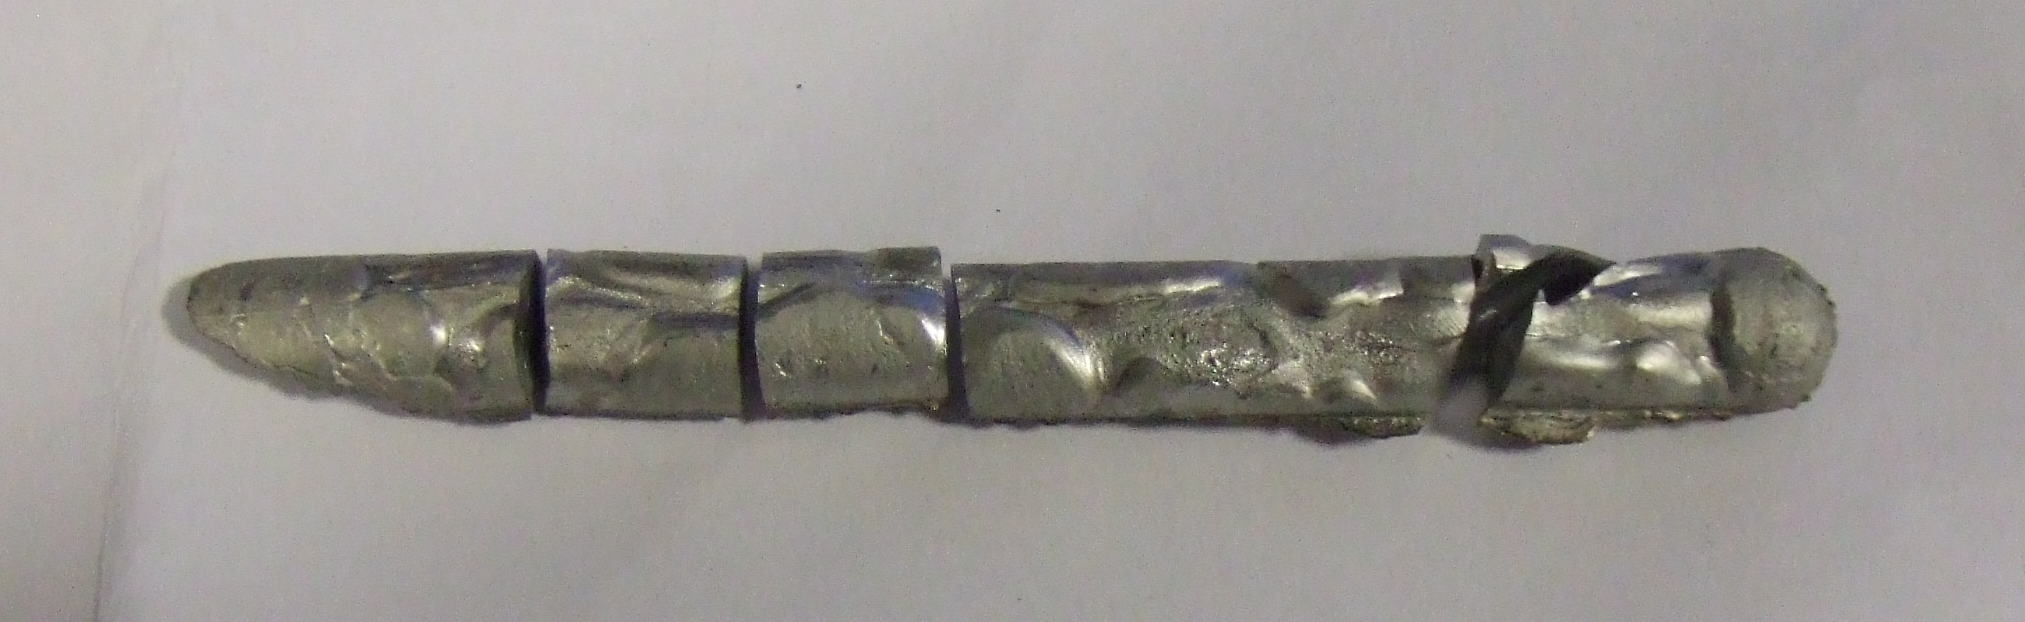
\includegraphics[width=10cm]{sanw_arc}
\caption{(a) An arc-melted ingot of \ilovewill{山}W using PM-manufactured feedstock.  It broke into several pieces on the water-chilled hearth when cooling down from melt temperature.}
\label{fig:sanw_arc}
\end{center}
\end{figure}
%

%
\begin{figure}[H]
\begin{center}
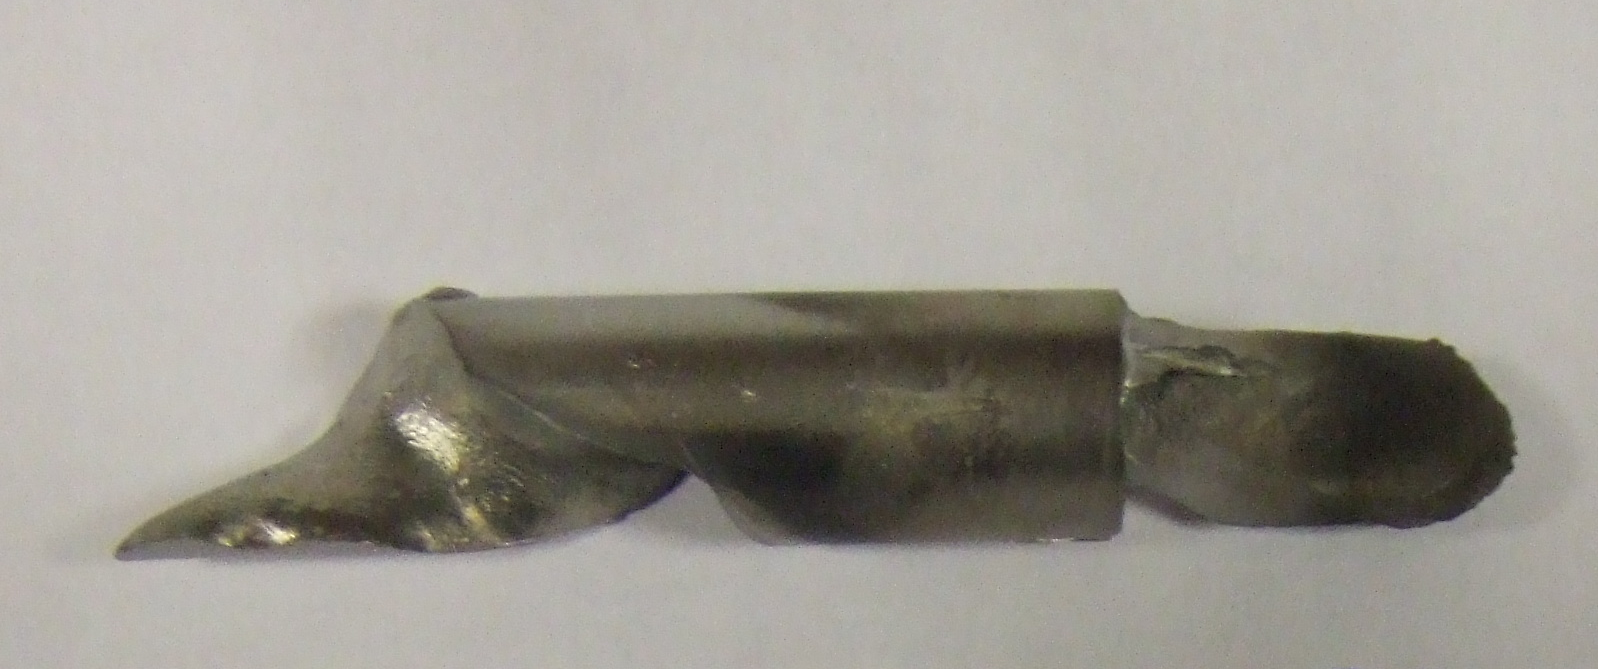
\includegraphics[width=10cm]{sanw}
\caption{(a) the long view of an ingot of DS manufactured \ilovewill{山}W using the in-house RF furnace, made with PM manufactured feed-stock. This was melted at about 1780\celsius\ and drawn at 30milli\metre\/h. Part-way through the cast, the thermocouple broke, and the furnace was run at maximum capacity to increase the chances of a successful cast.}
\label{fig:sanw}
\end{center}
\end{figure}
%


\clearpage
\subsection{Four-Mirror Image Furnace Manufacture}

Several casts was performed using the 4-mirror furnace at the Physics Department of the University of Warwick (Figure \ref{fig:MirrorFurnace}).  This method of casting has been successfully used to manufacture single-crystal single-phase intermetallics and ceramics.  A homogeneous, single-phase feed ingot with a circular cross-section is required.  Feed ingots are typically made via the arc-melt process or through pressing powders.  The seed ingot needs to be single-crystal to manufacture single-crystal material.  

This method has not been successfully used to manufacture eutectic alloys.  Slight deviations from eutectic composition in the feed ingot would result in substantial temperature fluctuations in the melt.  If the composition being melted has a too high of a melting point due to the presence of primary dendrites, the melt volume would shrink and contact between the feed ingot and seed ingot would break. 
 

The casting rate was at the furnace's maximum drawing rate of 18 mm/h.  Despite using an ingot that had undergone several arc-melts, inhomogenities still persisted, and the melt could not be sustained as the melting temperature of the feed ingot fluctuated too much.  Due to the unstable nature of casting inhomogeneous eutectic alloys, the melt broke three times.  Although melt contact was re-established each time, this meant that the grains were discontinuous, and there is not enough uninterrupted length to machine out a creep specimen (Figure \ref{fig:FirstCast}).

At this casting rate, a lamellar microstructure should be seen.  However, there is too much dendritic chromium solid-solution pro-eutectic in the microstructure disrupting lamellae formation.  Only about 2\% of the area fraction of the transverse section was lamellar. 
%
\begin{figure}[H]
\begin{center}
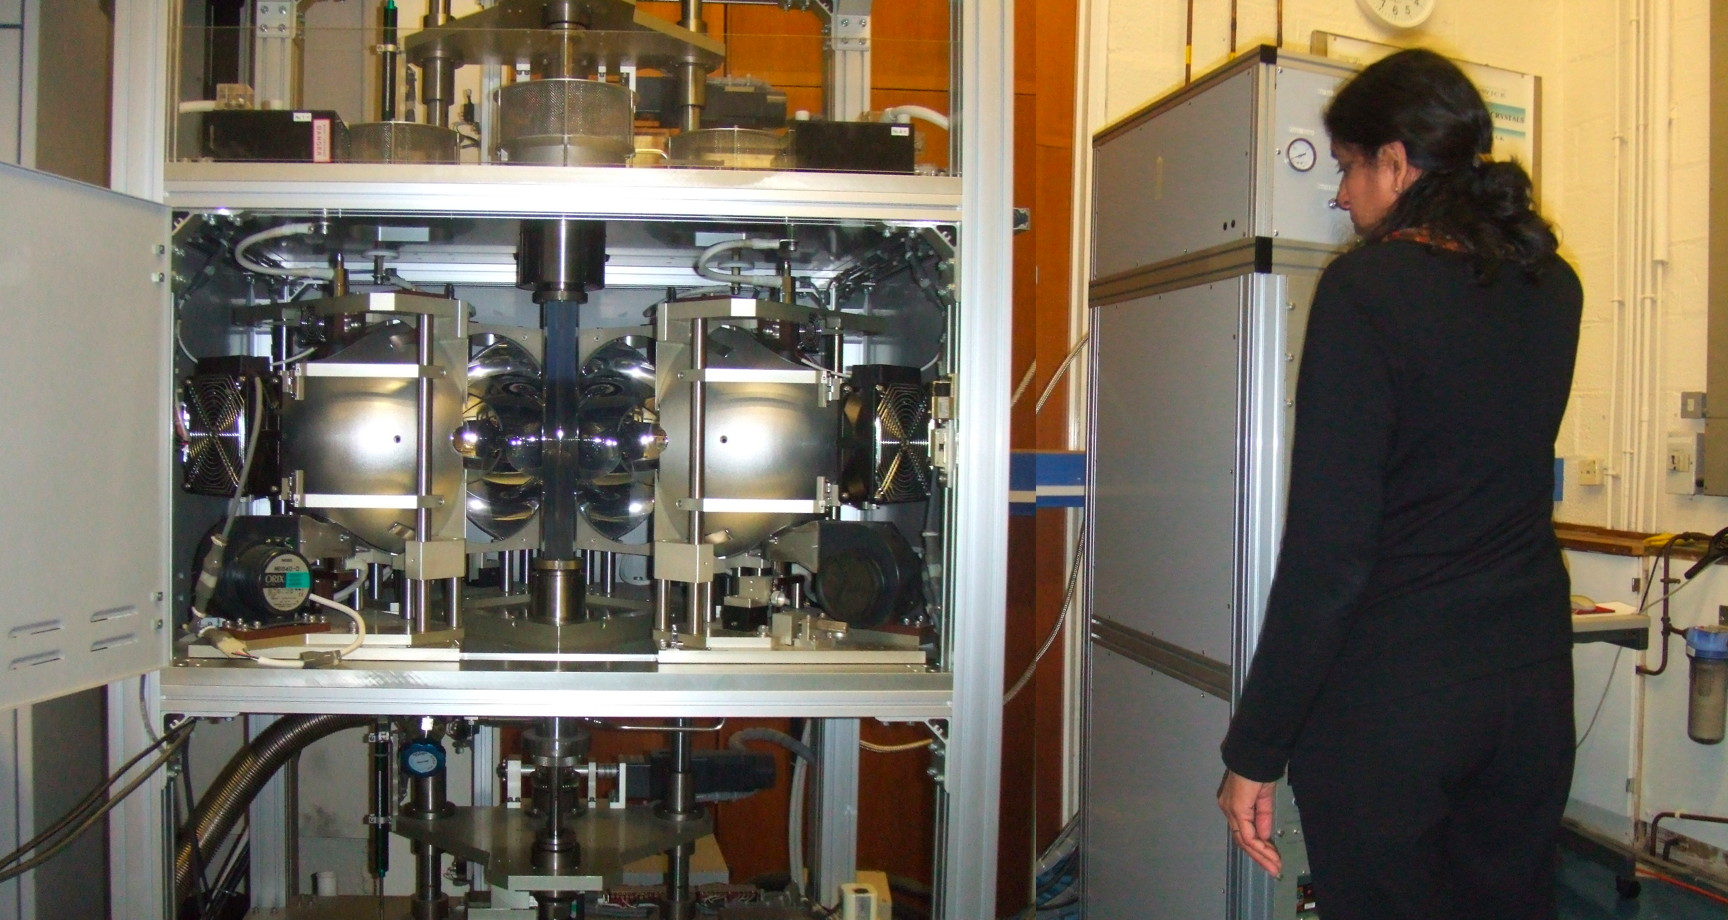
\includegraphics{MirrorFurnace}
\caption{Photograph of the 4-mirror furnace at the University of Warwick.}
\label{fig:MirrorFurnace}
\end{center}
\end{figure}
%
%
\begin{figure}[H]
\begin{center}
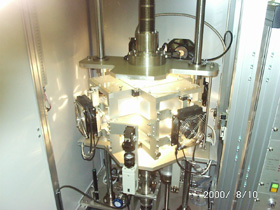
\includegraphics{mirroron}
\caption{Photograph of the 4-mirror furnace in operation.}
\label{fig:MirrorFurnace}
\end{center}
\end{figure}
%

%
\begin{figure}[H]
\begin{center}
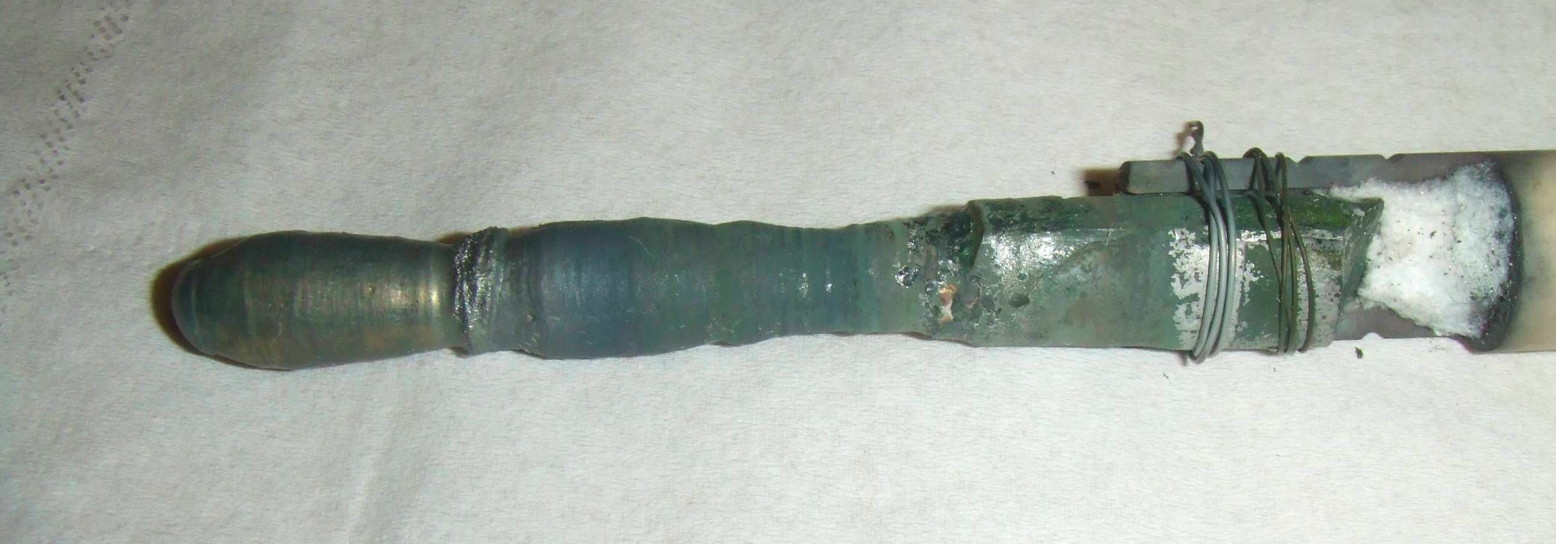
\includegraphics{FirstCast}
\caption{Photograph of the first directionally solidified Cr--Cr$_3$Si ingot.}\label{fig:FirstCast}
\end{center}
\end{figure}
%



